% ------------------------------------------------------------------------------
% LaTeX Template: Titlepage
% This is a title page template which be used for both articles and reports.
%
% Copyright: http://www.howtotex.com/
% Date: April 2011
% ------------------------------------------------------------------------------

% -------------------------------------------------------------------------------
% Preamble
% -------------------------------------------------------------------------------
\documentclass[paper=a4, fontsize=11pt,twoside]{scrartcl}		% Koma article

\usepackage[a4paper,pdftex]{geometry}										% A4paper margins
\setlength{\oddsidemargin}{5mm}												% Remove 'twosided' indentation
\setlength{\evensidemargin}{5mm}
\usepackage{graphicx}
\usepackage{multirow}
\usepackage{chngpage}
\usepackage{array}
\usepackage{supertabular}
\usepackage{extramarks} % Required for headers and footers
\usepackage{float}
\usepackage[english]{babel}
\usepackage[protrusion=true,expansion=true]{microtype}	
\usepackage{amsmath,amsfonts,amsthm,amssymb}
\usepackage{graphicx}
\usepackage[nottoc,numbib]{tocbibind} % Required for inlucde reference in TOC
\usepackage[pdfstartview=FitH,
	CJKbookmarks=true,
	bookmarksnumbered=true,
	bookmarksopen=true,
	colorlinks,
	linkcolor=black,
	citecolor=blue,
]{hyperref} % Required for hyper link references

\usepackage[numbers,sort&compress]{natbib}
\usepackage{CJK}
\usepackage{algorithm}
\usepackage{algorithmicx}
\usepackage{algpseudocode}
\usepackage{amsmath}

\usepackage{listings}
\usepackage{color}

\definecolor{dkgreen}{rgb}{0,0.6,0}
\definecolor{gray}{rgb}{0.5,0.5,0.5}
\definecolor{mauve}{rgb}{0.58,0,0.82}

\lstset{frame=tb,
  language=Java,
  aboveskip=3mm,
  belowskip=3mm,
  showstringspaces=false,
  columns=flexible,
  basicstyle={\small\ttfamily},
  numbers=none,
  numberstyle=\tiny\color{gray},
  keywordstyle=\color{blue},
  commentstyle=\color{dkgreen},
  stringstyle=\color{mauve},
  breaklines=true,
  language=Java,
  breakatwhitespace=true,
  tabsize=3
}

% ------------------------------------------------------------------------------
% Definitions (do not change this)
% ------------------------------------------------------------------------------
\newcommand{\HRule}[1]{\rule{\linewidth}{#1}} 	% Horizontal rule

\makeatletter							% Title
\def\printtitle{%						
    {\centering \@title\par}}
\makeatother									

\makeatletter							% Author
\def\printauthor{%					
    {\centering\large \@author}}				
\makeatother							

% ------------------------------------------------------------------------------
% Metadata (Change this)
% ------------------------------------------------------------------------------
\title{	\LARGE \textbf{AE2GRP Final Group Report} 	% Subtitle of the document
		 	\\[2.0cm]													% 2cm spacing
			\HRule{0.5pt} \\										% Upper rule
			\LARGE \textbf{\uppercase{Animation of Sorting Algorithms}}	% project title
			\HRule{2pt} \\ [0.5cm]								% Lower rule + 0.5cm spacing
			\normalsize \today									% Todays date
		}

\author{
\begin{tabbing}
      \hspace{5.1cm}\= \textbf{Group ID:} \quad\quad\= 5\\
      			  \>\textbf{Group Members: }\\ 
                  \\
                  \> Jiaying SUN       \> 6515778\\
                  \> Kan LIU     	   \> 6515770\\
                  \> Muyi JIANG        \> 6513225\\
                  \> Yangyu GAO        \> 6515761\\
                  \> Zhefeng ZHOU      \> 6515792\\
                  \> Zhe REN      	   \> 6515775
    \end{tabbing}
				\textbf{Supervisor: } Heshan DU\\	
        }
    
\begin{document}
% ------------------------------------------------------------------------------
% Maketitle
% ------------------------------------------------------------------------------
\thispagestyle{empty}				% Remove page numbering on this page
\printtitle									% Print the title data as defined above
  	\vfill
\printauthor								% Print the author data as defined above
\cleardoublepage

% ------------------------------------------------------------------------------
%  table of contents
% ------------------------------------------------------------------------------
\newpage
\tableofcontents
\thispagestyle{empty}	
\newpage
\cleardoublepage

% ------------------------------------------------------------------------------
% Begin document
% ------------------------------------------------------------------------------

\setcounter{page}{1}

% ------------------------------------------------------------------------------
% INTRODUCTION      Kan LIU
% -----------------------------------------------------------------------------

\section{Introduction}

\subsection{Project Introduction}
Most beginners of computer science need to learn sorting algorithms. A sorting algorithm is a sequence of steps which provides a solution to sorting problems. Sorting is often used in our daily life. For instance, if teachers need to enter students' exam marks by student IDs to make the process of entering marks easier, they can use sorting algorithms to sort answer sheet first. Sorting algorithms are an essential part of algorithms and data structures. By learning sorting algorithms, people can save time when solving sorting problems. However, sorting algorithms are challenging to understand by only reading the descriptions in pseudo-code or programming languages. It is necessary to find some methods to enable more efficient ways of learning sorting algorithms.\\

\textbf{The problem} that this project aims to solve is:``How to develop a software tool to help people learn sorting algorithms more efficiently.''\\

To solve this problem, we find that visualization is a useful tool. It describes the execution of sorting algorithms as a continuous sequence of graphical images. Michael claims that animations help people remember algorithms better, because they explain a dynamic, evolving process clearly \cite{Intro.2}. Lawrence, Badre, and Stasko utilized animations to help teach undergraduates about minimum spanning tree algorithms in 1994 \cite{Intro.3}. A significant benefit was found when students could interact with the algorithm animations in a laboratory context. In this project, we will develop a creative open-sourced software to visualize sorting algorithms. This software should help people understand the correctness and efficiency of the sorting algorithms, facilitate learning and increase the interest of people. 


\subsection{Team Introduction}
Our team consists of five Computer Science undergraduates from University of Nottingham Ningbo China. All the five students are in Part I.

\begin{table}[H]
\caption{Team Role}
\begin{center}
\begin{tabular}{|l|l|}
\hline
\multicolumn{1}{|c|}{\textbf{Name}} &
\multicolumn{1}{|c|}{\textbf{Role}}\\
\hline 
\textbf{Zhefeng Zhou} & Leader, User Experience Designer\\
\hline
\textbf{Yangyu Gao} & Quality Assurance Manager, Animation Expert\\
\hline
\textbf{Jiaying Sun} & Implementer \\
\hline
\textbf{Zhe Ren} & User Interface Designer    \\
\hline
\textbf{Kan Liu} & Editor   \\ 
\hline
\textbf{Muyi Jiang} & Repository Manager, Implementer   \\
\hline
\end{tabular}
\end{center}
\end{table}

As shown in Table 1, Different roles are allocated to team members. Zhefeng Zhou is our leader to coordinate work activities and he perform as User Experience (UX) Designer to concern with improving user experience. Yangyu Gao is the Quality Assurance (QA) Manager, who establishes procedures and quality standards and monitors these against agreed targets. Zhe Ren as the User Interface (UI) Designer designs the user interface of the software. Kan Liu as the Editor produces documents and makes sure all the key actions of our project are recorded. Muyi Jiang is the Repository Manager who manages the repository in GitHub and maintains codes and documentations  of our project. In addition, Jiaying Sun and Muyi Jiang are Implementer. 

\subsection{Introduction of Sorting Algorithm}

In this section, the basic knowledge of six sorting algorithms implemented in the software will be introduced. For each of the six sorting algorithms, the input is an unordered sequence, and the output is an ascending order sequence.\\
\begin{enumerate}
\item Bubble Sort\\
Bubble sort is a simple sorting algorithm. It repeatedly visits the sequence to be sorted, compare each pair of adjacency elements at a time, swap them if they are in the wrong order. The work of visiting the sequence is repeated until no swaps are required, which indicates the sequence has been sorted. The time complexity of bubble sort algorithm is $O(n^{2})$.

\item Insertion Sort\\
Insertion sort usually applies to sort small amounts of data. It works by building an ordered sequence, scan in the sorted sequence from the back to the front, find the appropriate location and insert for unordered data. Insertion sorting usually uses in-place sorting, so in the process scanning from the back to front, it needs to repeatedly shift the sorted elements gradually backward, to provide insertion space for the latest elements. The time complexity of insertion sort algorithm is $O(n^{2})$.

\item Selection Sort\\
Selection sort works as follows. First find the smallest element in the unordered sequence, store it at the beginning of the sorted sequence, and then continue looking for the smallest element from the remaining unordered elements, store it at the end of the sorted sequence. And so on until all the elements are sorted. The time complexity of selection sort algorithm is $O(n^{2})$.

\item Quick Sort\\
Quick sort is a randomized sorting algorithm based on the divide-and-conquer paradigm.
"Divide" means that divide sequence into three parts which is L, E and G by pick a pivot x. The elements in L is less than x, and the elements in E is equal to x, meanwhile the elements in G is greater than x. "Conquer" means join L, E and G together. The basic idea of quick sort is, first call the "Divide" operation on the unsorted sequence to get L, E and G parts. Then recursively call the "Divide" operation on L and G parts until the size of L and G is equal to zero or one. Finally, recursively invoke "Conquer" operation to join L, E and G parts to obtain an ordered sequence. The time complexity of quick sort algorithm is $O(n\log_{}n)$.

\item Merge Sort\\
Merge sort is a stable sorting algorithm, and it is an effective sorting algorithm based on merge operations, which applies "Divide and Conquer". The basic idea is merge the ordered subsequences to obtain a fully ordered sequence. In other words, data in each sub-sequence is ordered first, and then the sub-sequences are ordered. The time complexity of merge sort algorithm is $O(n\log_{}n)$.


\item Heap Sort\\
Heap sort is implemented by using heap data structure. A Heap is a complete binary tree, and it includes maximum heap and minimum heap. We introduce maximum heap as an example. The requirement for a maximum heap is that the value of each node is not greater than the value of its parent node, which means the maximum value is at the top of heap. The basic idea of heap sort is, first adjust the unsorted sequence to a maximum heap, next exchange the element of maximum value with the element at the end of sequence, then repeat the above two steps until all the elements are sorted. The time complexity of heap sort algorithm is $O(n\log_{}n)$.

\end{enumerate}
 

% ------------------------------------------------------------------------------
% Background Research   Kan LIU, Jiaying SUN, Zhe REN
% ------------------------------------------------------------------------------
\section{Background Research}
This part provides the background information and research of the software we developed. Section 2.1 describes similar systems, address some possible problems in the system design and discuss the market prospect of the software. Section 2.2 discusses which platform and tools are more suitable for this project. Section 2.3 talks about possible use cases.

\subsection{Existing Similar Systems and Market Research}

There are a few similar systems which provide the visualization of sorting algorithms. Three typical examples on the web, Visualgo\footnote{\url{https://visualgo.net/sorting}}, Algomation \footnote{\url{http://www.algomation.com/ and Algorithm}},  Visualizer\footnote{\url{http://algo-visualizer.jasonpark.me}} and Sorting Algorithms Visualizer, are described in this section. The first two applications are based on the Web. The third one is based on the Windows system. \\

\textbf{SortingVisualization}
\begin{figure}[htbp]
    \centering
    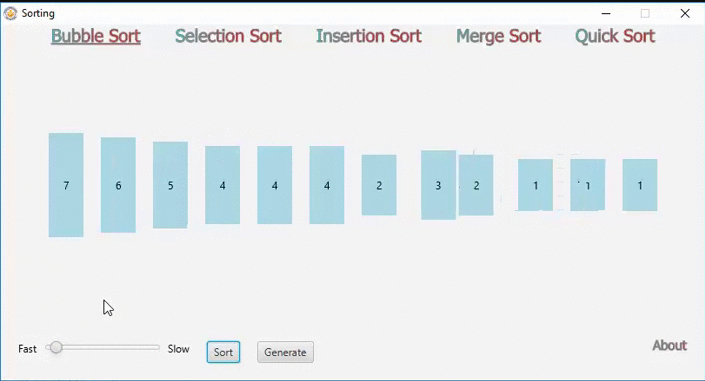
\includegraphics[width=.8\textwidth]{SortingVisual.png}
    \caption{SortingVisual}
    \label{fig:sortingVisual}
\end{figure}

SortingVisualization is a simple JavaFx application that visualize the common sorting algorithms through animations, 


\textbf{Visualgo}\\
\begin{figure}[htbp]
\centering
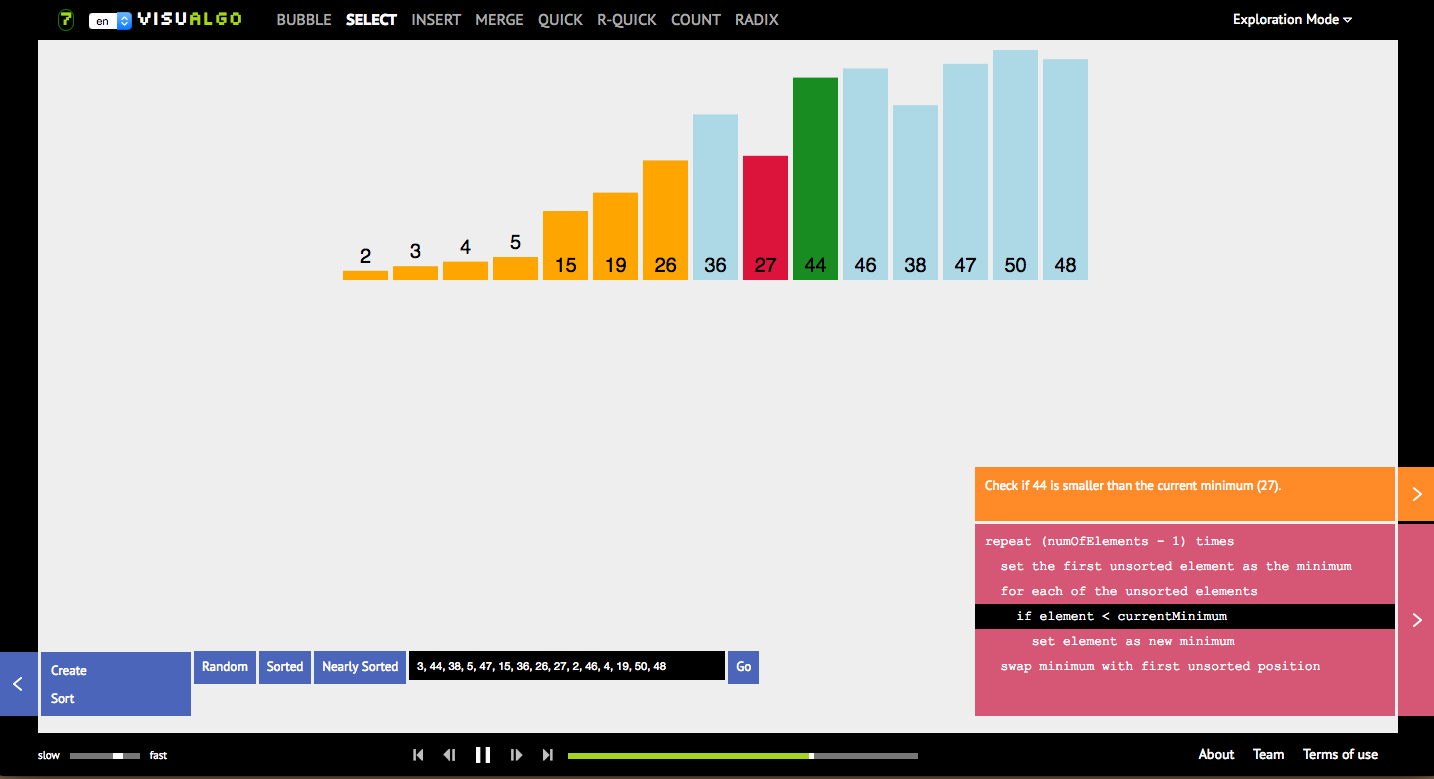
\includegraphics[width=.8\textwidth]{Visualgo.png}
\caption{Visualgo}
\label{Visualgo}
\end{figure}

Visualgo was conceptualized in 2011 by Dr.Steven Halim as a tool to help his students to have a better understanding of data structures and algorithms. It is specifically designed for National University of Singapore (NUS) students taking data structure and algorithm classes. This software centers around teaching students the principles of algorithms. As is shown in Figure \ref{Visualgo}, it contains numerous useful functions. Firstly, the user interface is beautiful as the color of operating block can be changed when users refresh the page. In addition, this system can generate graphical images for random input data or that specified by users. Thirdly, when the animation plays, the pseudo code and explanation of corresponding steps will be shown in the low right corner. This makes users understand an algorithm more easily. However, there are some shortcomings. Some space is not well utilized, such as the space below the animation. The ``Start Button'' is so small that people might confuse how to start the animation. Similarly, the user guide is in the high right corner which is inconspicuous and users might not know where it is.\\ \\


\textbf{Algomation}\\

\begin{figure}[htbp]
\centering
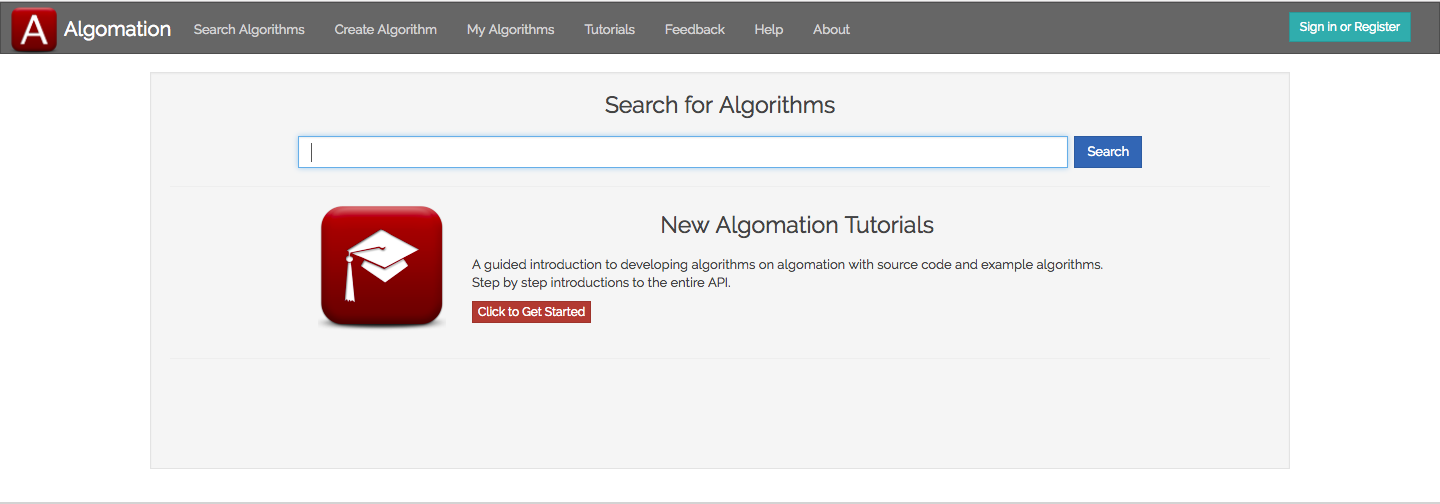
\includegraphics[width=.8\textwidth]{searchAlgomation.png}
\caption{searchAlgomation}
\label{searchAlgomation}
\end{figure}

\begin{figure}[htbp]
\centering
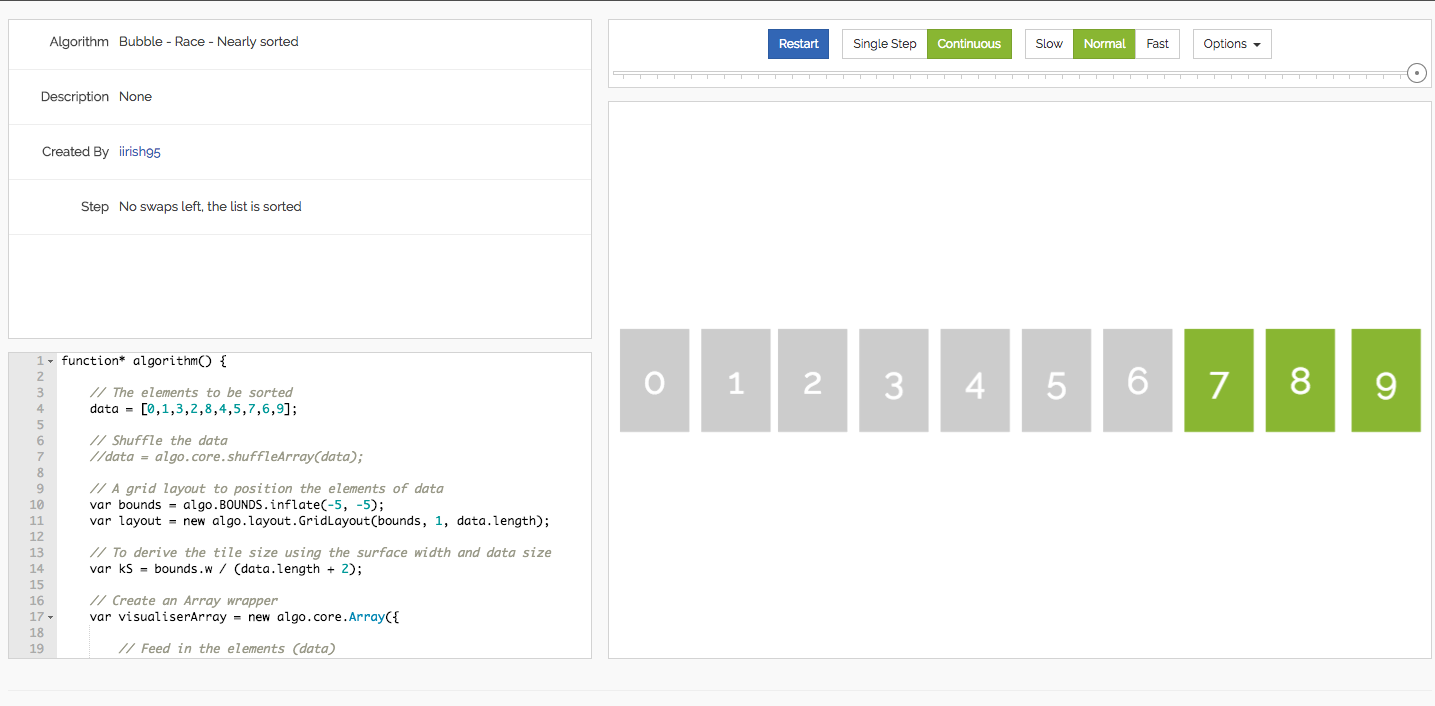
\includegraphics[width=.8\textwidth]{Agomation.png}
\caption{Agomation}
\label{Agomation}
\end{figure}


Algomation is a platform for viewing, creating and sharing any type of algorithm. All algorithms on the site are public and can be viewed and shared by any user of the site. This website is created by Duncan Meech. As the Figure \ref{searchAlgomation} shown, users can search algorithms they want in this website. After selecting an algorithm, the player page will be shown in the Figure \ref{Agomation} which incorporates four main components: Player Visualizer, Player Controls, Player Source code Viewer and Player Message. The Player Visualizer is in the right part to display the anamation. The Player Controls is above the animation part to control the animation which can change the mode and speed of animation, share to other people, restart the animation and so on. There are a message part in the upper right hand to describe the message about the visualization such as the author. The last part is in the low right hand to provide the source code. It is more convenient for users to understand the algorithm. There are many useful algorithms with different types of animations in the website. There are also lots of useful functions to help people learning. Moreover, The difference between other software is that people can get tutorial of developing algorithm animations. They can develop a animation to help learn algorithm. \\



\textbf{Algorithm Visualizer}\\
\begin{figure}[htbp]
\centering
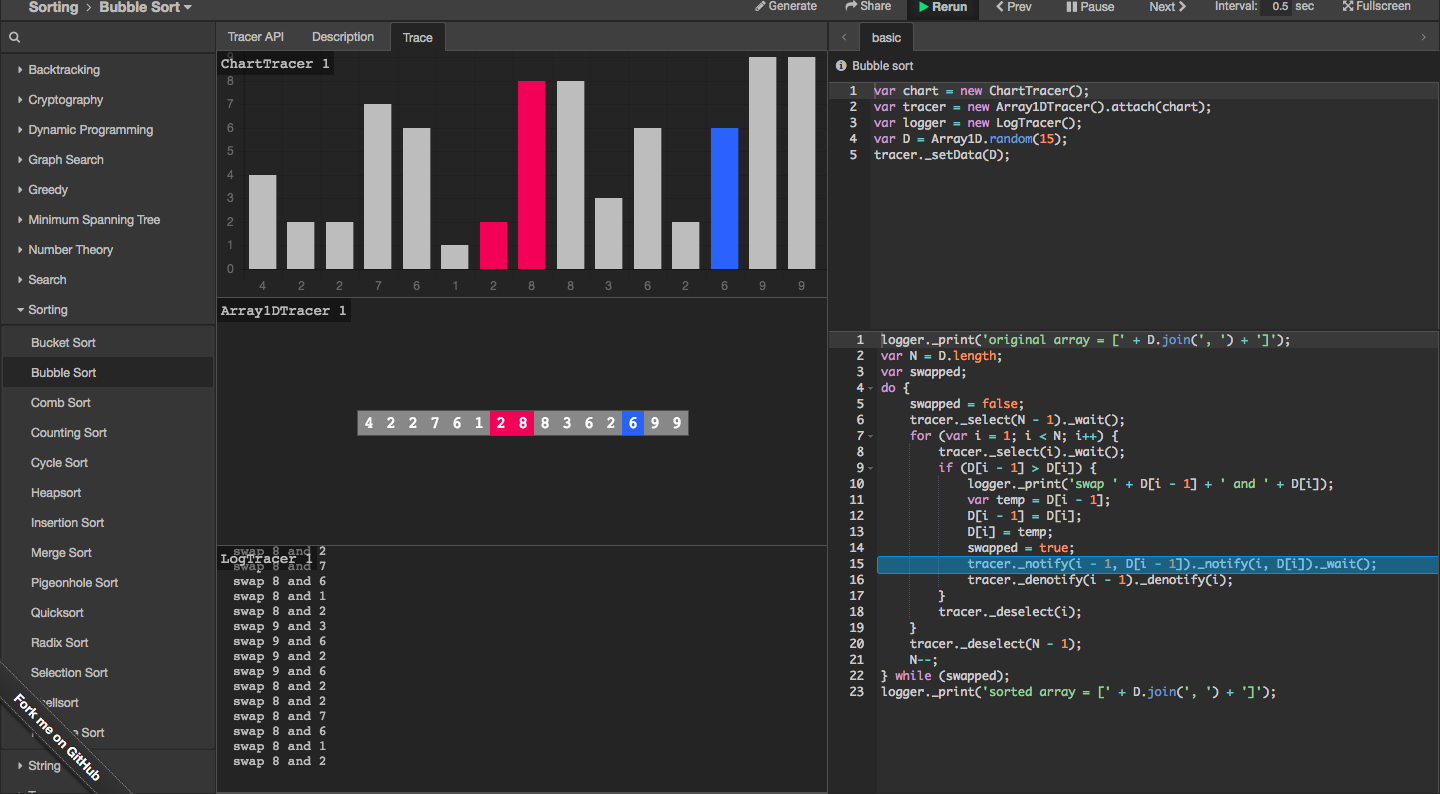
\includegraphics[width=.8\textwidth]{algo-visualizer.png}
\caption{Algorithm Visualizer}
\label{Algorithm Visualizer}
\end{figure}

Algorithm Visualizer is an open-source software which is developed by Jason Park and others. This software concentrates on visualizing a single sorting algorithm. It is composed of several blocks which are shown in Figure \ref{Algorithm Visualizer}. The left side is a list of different algorithms users can choose. The middle part shows two visualizations, ChartTracer 1 and Array1DTracer 1, with the different forms which can meet different needs. LogTracer 1 shows some information to explain each step. On the right side, the whole block displays the JavaScript code of this sorting algorithm. Users can modify the code to change input of animations. By checking the actual code of animation, the learning interest of users might grow. \\


\textbf{Sorting Algorithms Visualizer}\\
\begin{figure}[htbp]
\centering
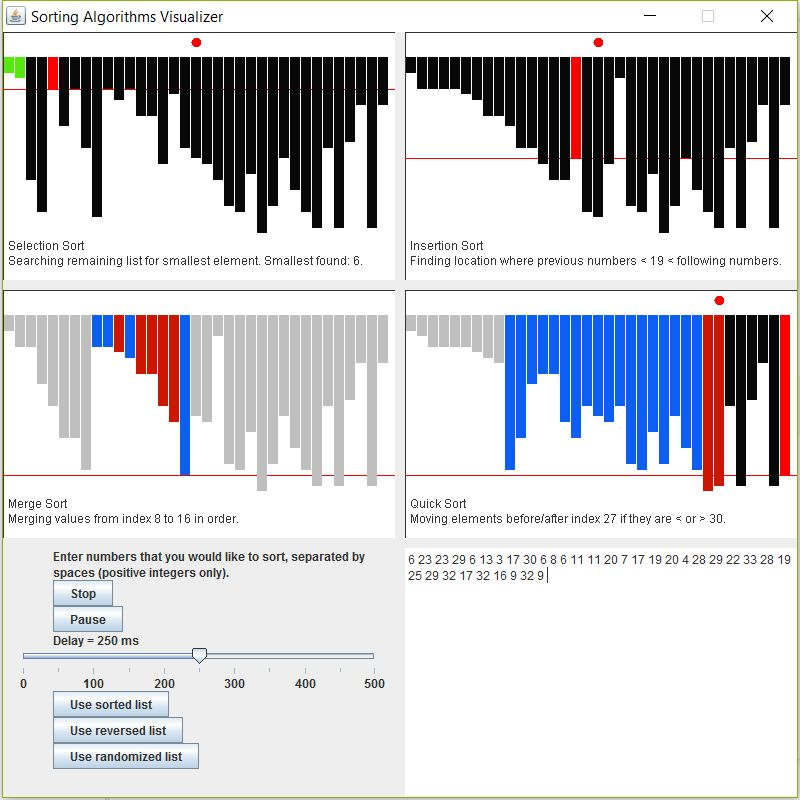
\includegraphics[width=.6\textwidth]{SortingAlgorithmvisualizer.JPG}
\caption{Sorting Algorithms Visualizer}
\label{SortingAlgorithmvisualizer}
\end{figure}

Sorting Algorithm Visualizer is a software based on the Windows system which is shown in Figure \ref{SortingAlgorithmvisualizer}. Differring from the former two systems, this system focuses on comparing the efficiency of different sorting algorithms. The user interface of this software is succinct. There are also some explanations below each animation. Users can specify inputs by choosing a sorted list, a reversed list or a randomized list. Users also can specify inputs by themselves. However, this software is not very stable and may fail unexpectedly. Moreover, only four sorting algorithms are supported by the system. Users may want to learning more sorting algorithms.

Compared to other similar systems, our system will have three advantages. First, as an open-source software, everyone can use it. Secondly, our system is based on the Windows system and can be used without the Internet. Thirdly, most similar software only focus on the animation of sorting algorithms rather than comparing the efficiency of them. Our software will not only concentrate on single algorithm but also provide the comparison of sorting algorithms. 

\subsection{Technical Research}

\begin{enumerate}
	\item \textbf{GUI Design}\\
    There are many frameworks to design GUI for Java. The Abstract Window Toolkit (AWT) is part of the Java Foundation Classes (JFC), the standard API for providing a graphical user interface (GUI) for a Java program. AWT is also the GUI toolkit for a number of Java ME profiles.Swing was developed to provide a more sophisticated set of GUI components than the earlier Abstract Window Toolkit (AWT). Swing provides a native look and feel that emulates the look and feel of several platforms, and also supports a pluggable look and feel that allows applications to have a look and feel unrelated to the underlying platform. JavaFX is another software platform for creating and delivering desktop applications, as well as rich internet applications (RIAs) that can run across a wide variety of devices. By using JavaFX, we can also use the web language (HTML, CSS and JavaScript) indirectly to make our interface more visual.

\begin{figure}[htbp]
\centering
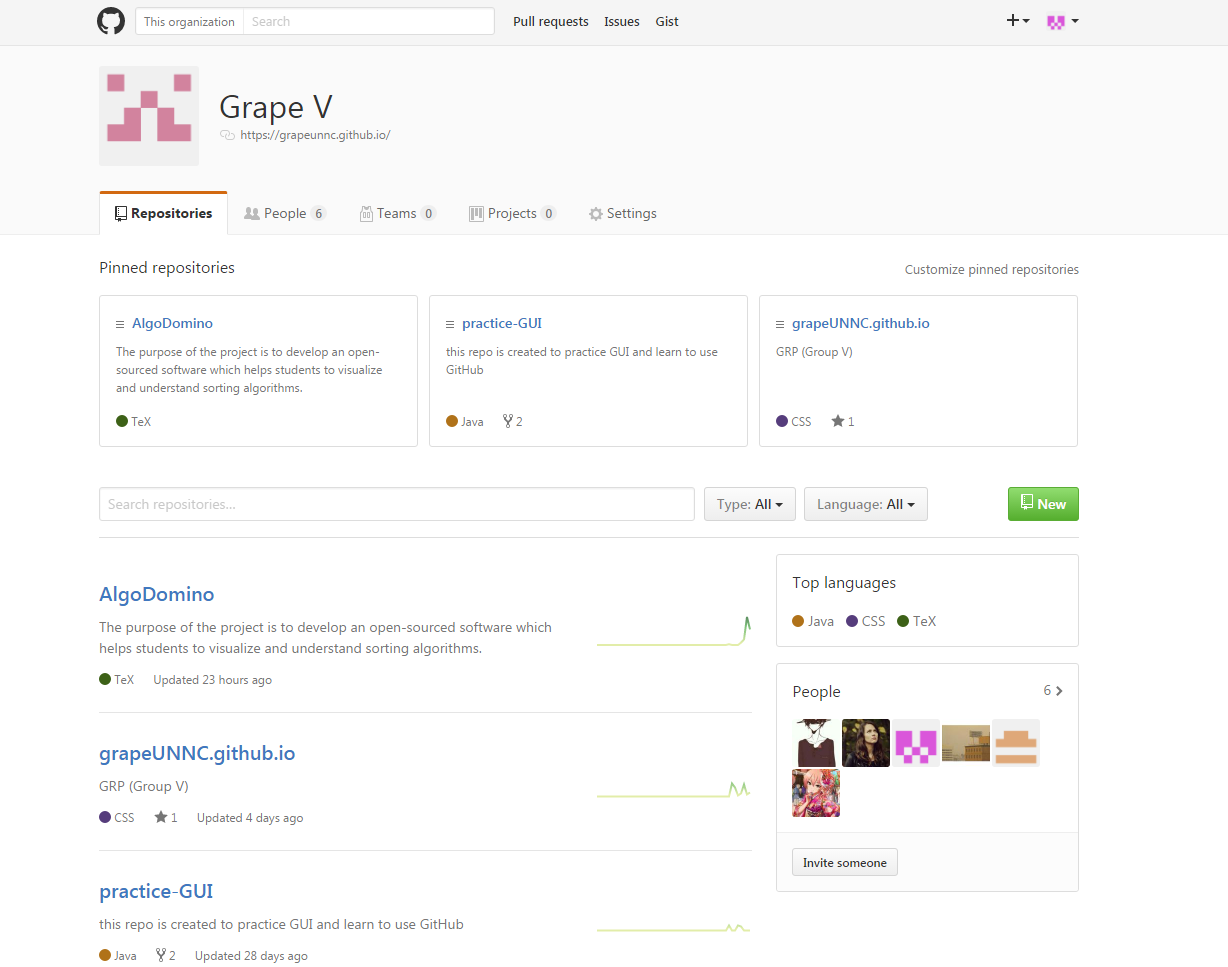
\includegraphics[width=.8\textwidth]{github.PNG}
\caption{Github page}
\label{github}
\end{figure}
	\item \textbf{Version control}\\
    Git is an distributed version control system, which can keep the history of a file set, and can roll back the file to another state (history). Github\footnote{\url{https://github.com}} is a git based web collaboration community. It can work as Git to keep the history of a file and roll back the file state, and have a variety of mechanisms for everyone to work together to contribute to the project. In addition, Github integrates lots of social features which make users` information and activities visible across open source software projects \cite{dabbish2012social}. Our group decides to use Github as a basic tool to develop the software, so that we can upload the software project to a repository where everyone can access and work on it, control the project versions, and search some useful open resource distributed in Github. 

	\item \textbf{Animation}\\
The most common way to animate nowadays is using Javascript or CSS. There are many good JavaScript animation libraries on the market, and each
of them has specific different features. Each project has its own requirements,
but sometimes one library is not sufficient to meet the whole requirements of one
project. Some famous and powerful JavaScript libraries are GSAP\footnote{\url{http://greensock.com/gsap}}, Velocity.js\footnote{\url{http://velocityjs.org/}} and jQuery\footnote{\url{http://jquery.com/}}.

	
\end{enumerate}


\subsection{Use Cases}
It is necessary to find several use cases for our software to plan the goals of the next stages. Here are some possible use cases.
\begin{enumerate}
\item \textbf{Teaching}\\
This software may be used as a convenient tool for teaching. For example, when teachers in class want to teach sorting algorithms, they can use our software to explain the principles. Students would understand them more easily.

\item \textbf{Self-study}\\
Some people may need to learn sorting algorithms. However, they do not have a teacher and they cannot understand sorting algorithms searched from online. This software becomes a good helper to explain knowledge by visualization.

\item \textbf{Review}\\
People may forget the knowledge they have learned. By using this software, they can revise the sorting algorithms. The comparison of the efficiency of different algorithms would help users learn or reuse the algorithms more quickly.
\end{enumerate}


% ------------------------------------------------------------------------------
% Requirement Specification
% ------------------------------------------------------------------------------

\section{Requirement Specification}

This section specifies the requirements for our software. As mentioned before, the purpose of this software is to help users learn principles and efficiency of sorting algorithm. Hence, users should have a basic understanding of what an algorithm is. Typical users include computer science students and those interested in sorting algorithms. The rest of this section presents the specifications of the software. The first part is an overall description of the software and its functional requirements. The second part outlines other related non-functional requirements of the software.   

\subsection{Functional Requirements}

The list provides a description of main functional features. These features are divided into two categories: core features and optional features. Core features are essential to the operation of the software and optional features are additional functionality.\\

\textbullet{\textbf{ Core features}}

\begin{enumerate}
\item The software should provide users a guide of how to use core features.  

\item The software should allow users to select which sorting algorithms to animate.

\item The software should be able to allow users to define input data by themselves.

\item The software should be able to generate input data randomly.
                                                    
\item The software should be able to visualize the processes of running a sorting algorithm. 

\item The software should allow users to start, stop, slow down, speed up, restart or pick up a point of the animation.

\item The software should be able to show the running sorting algorithm's source code to users.

\item The software should be able to compare the efficiency of different sorting algorithms by  showing the animation simultaneously.

\item The software should allow users to select which algorithms to compare.

\item The software should be able to provide the time complexities of sorting algorithms when comparing the efficiency.


\end{enumerate}

\textbullet{\textbf{ Optional features}}

\begin{enumerate}
\item Users should be able to share the animation as video or gif file to some social network websites.

\item The software should allow users to customize the interface, such as the background color of animation, shapes and colors of basic components used in an animation.

\item Users should be able to download the source code of selected sorting algorithms in several programming languages such as Java, C, Python, JavaScript and PHP.

\end{enumerate}


\subsection{Non-functional Requirements}
\begin{enumerate}
\item Platform\\ The software will run on Windows, Mac and Linux with JRE (Java SE Runtime Environment).

\item Capacity\\The software allows users to compare two sorting algorithms only.

\item Software Language\\ All code will be written in Java SE8, JavaFx and CSS.  

\item Online User Documentation and Help System Requirements\\The software should allow users to download the source code to local address. All documentation will be made in accordance with requirements pertaining to open source software under the GNU General Purpose License. Additionally, online user documentation will be in the form of Java Platform, Standard Edition 8 API Specification.

\end{enumerate}


% ------------------------------------------------------------------------------
% Design      Muyi JIANG ,Yangyu GAO
% -----------------------------------------------------------------------------
\section{Design}
This section describes the design of the software. Section 4.1 presents two UML models of the design.  Section 4.2 shows the user interface design.

\subsection{UML Model}
The Unified Modeling Language (UML) is a visual, object-oriented, and multipurpose modeling language. It is primarily designed for modeling software systems \cite{Gregor20055}. From different perspectives of the system, UML defines use case diagram, sequence diagram, class diagram and so on. With UML, we can model the types, properties, and states of those objects as well as to integrate corresponding object flows into the activities \cite{Gregor20055}. In this part, we will analyze use case diagram and sequence diagram for our software according to the requirement specification.

\subsubsection{Use Case Diagram}
\begin{figure}[htbp]
\centering
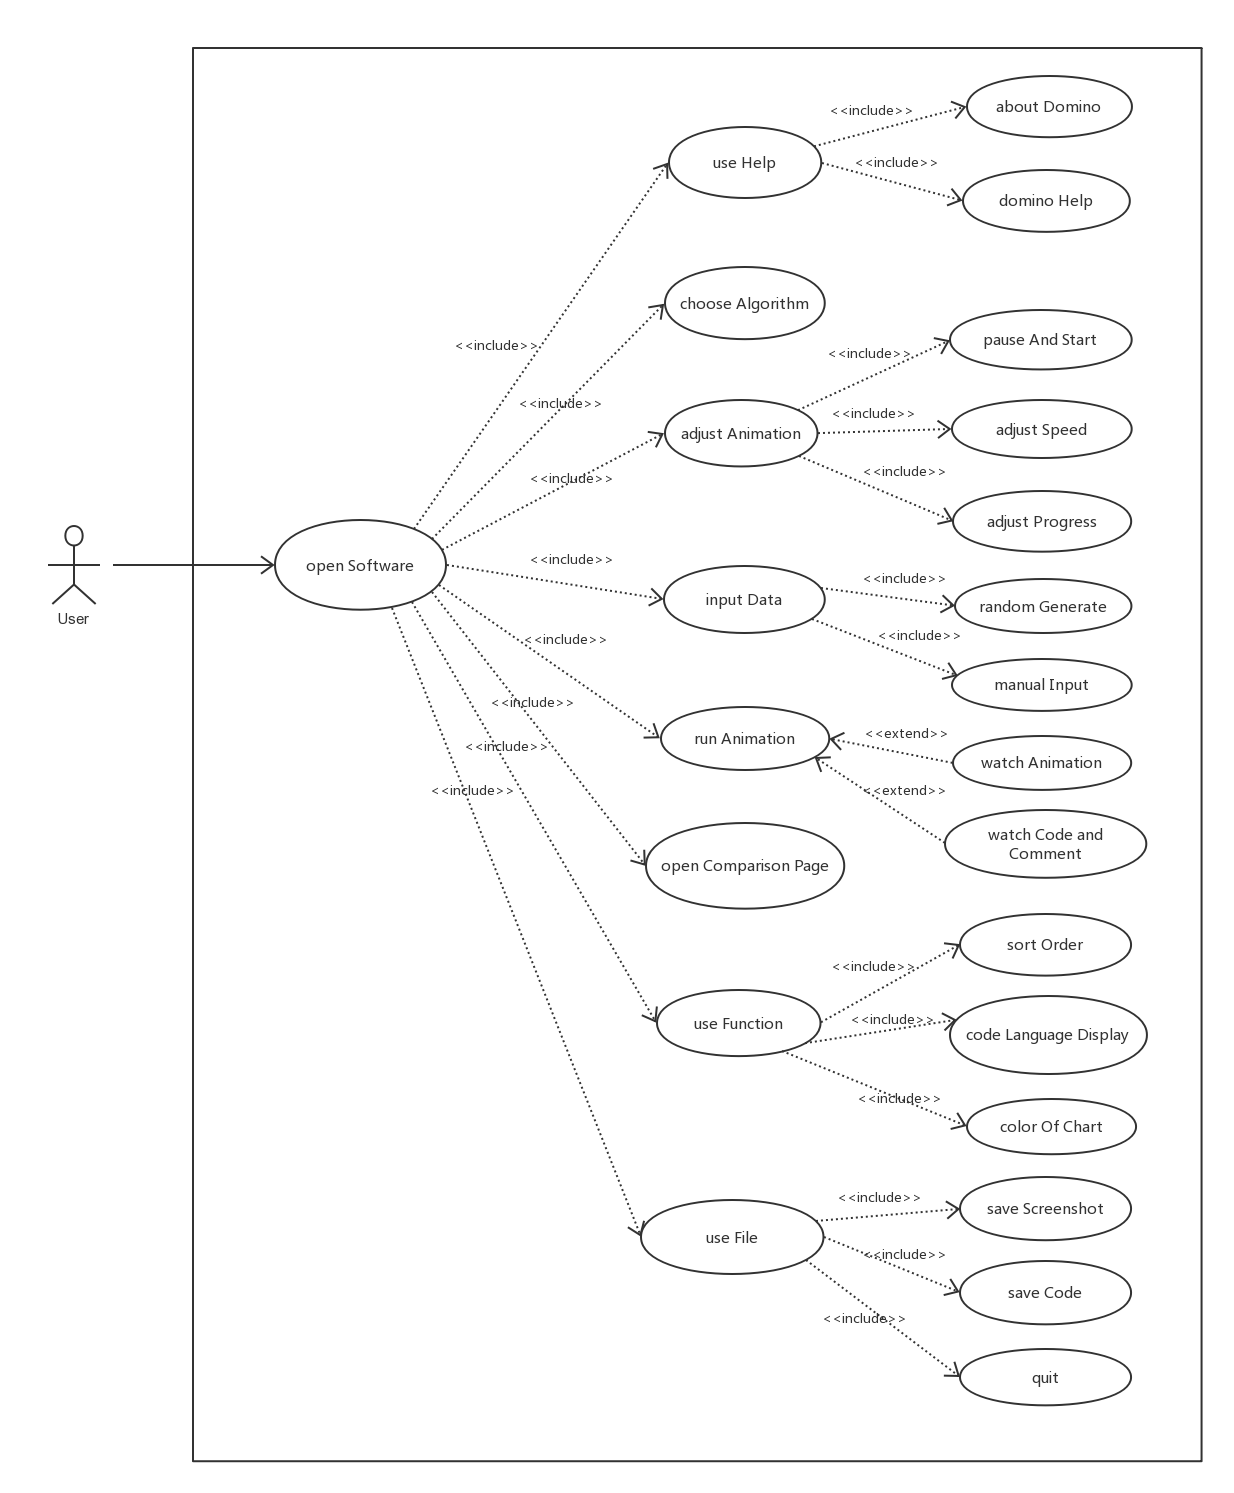
\includegraphics[width=1\textwidth,height=1.3\textwidth]{usecase.png}
\caption{Use case diagram}
\label{usecase}
\end{figure}
According to Wegmann and Genilloud, use case diagram is used to represent functions of the system \cite{Wegmann2000The}. The advantage of use case diagram is that it can describe the functions of software in a clear and visual way. Figure \ref{usecase} is a use case diagram drawn on the basis of the functional requirements of our software. From it we can see that every use case of the user is captured, and most of them can include or extend to different sub use cases. The diagram is designed to describe all the available functions when users open the software. We list some of the available functions as examples, such as users can choose six different sorting algorithms, users can click "start" button to run the animation, users can watch the animation and corresponding algorithm code, users can adjust the speed and the progress of animation, and users can use functions in menu bar such as "File", "Function" and "Help".
\subsubsection{Sequence Diagram}
\begin{figure}[htbp]
\centering
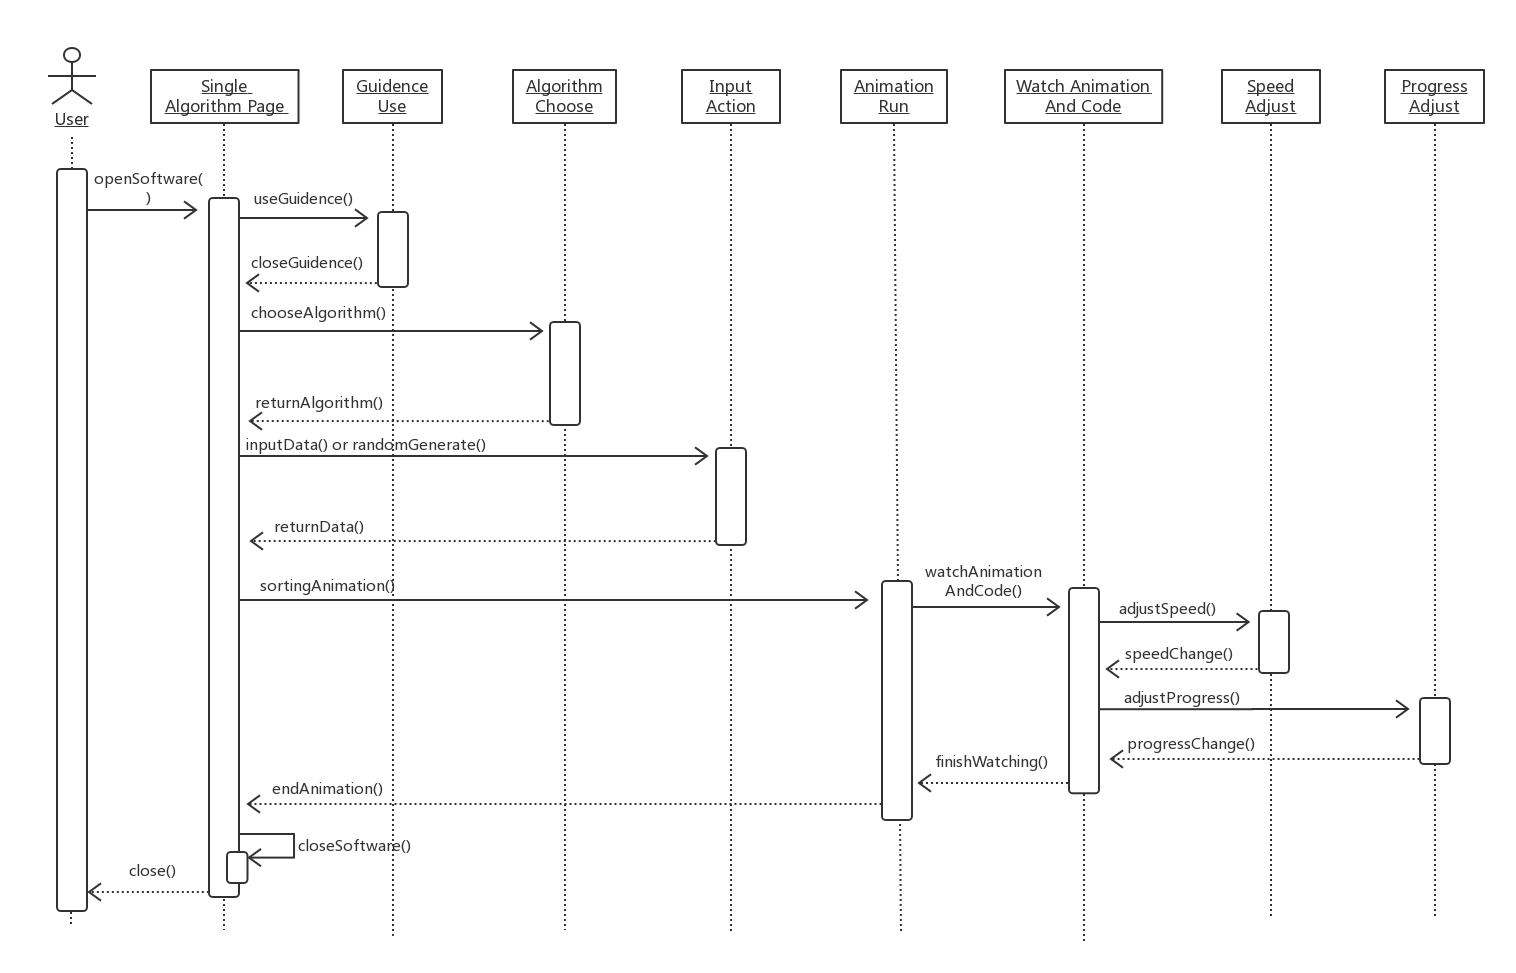
\includegraphics[width=1\textwidth,height=1.1\textwidth]{sequence.png}
\caption{Sequence Diagram}
\label{sequence}
\end{figure}
Bell claims that sequence diagram primarily shows the interactions between objects in the sequential order that those events occur \cite{Bell2005UML}. The advantage of sequence diagram is that it can clearly describe the time line of events happening and the interactions among objects. Figure \ref{sequence} is a sequence diagram drawn according to the functional requirements of our software. The diagram is designed to describe the sequence of events happening when a user uses the software to watch the animation of one sorting algorithm, first, when the user opens the software, he will first see the single algorithm page, then he finds the guidance to teach him how to use the software. After the guidance, he selects an algorithm and inputs specific data, next he runs the animation. During the animation, he watches the animation and corresponding algorithm code, meanwhile he adjusts the speed bar and progress bar of animation. Finally, he closes the software after watching the animation.

\subsection{User Interface Design}

In our initial design, we decided to put several functions into the user interface. The main part should be a block used for the animation. Since most of computer users watch video, we decided to add some functions similar with the video player. Therefore, we added play/pause button, progress bar, rewind and fast-forward button. We also decided to add some buttons to change the speed of animation. We add a choice box into the right-side block to let the users choose the algorithm. For generating image of animation, we add a block to let users input data so that the computer can use these numbers to generate a corresponding image. We also thought that a function comparing two algorithms’ animation is necessary and helpful, so we add a menu bar including some basic functions and the comparing functions. \\
During the process of developing, we found that the initial graphical user interface still has some defects. Some functions and layout designs are not interactive and friendly to users. For example, the original algorithm choosing function used only a choice box at the right side of the interface. But it will cause a lot of useless space in the right-side block. For the single algorithm animation, we want to add more user-defined options. But for the comparing function, we decide to add more analysis function into this part. Therefore, we try to create two interfaces for these functions to make the software more convenient. In single algorithm interface, we decide to create a special algorithm choosing function which seems like choosing page in power point. Users can also overview the simple animation of every algorithm. This design is more interactive and can enable a better user experience. Another problem is the input block. Since this part has a strange position which don’t contribute to a tidy interface, we need to relocate this function and adjust some other parts. The speed button seems convenient to use, but it’s not user-friendly enough. So we try to use the speed bar to replace that. We also decide to separate out the page swapping function from the menu bar so that users can use this function more conveniently. We also try to add more functions in the menu bar to make the whole software more interactive and complete.


\subsubsection{Menu Bar}
The software includes three menus, each of which implements basic functions.  
\begin{enumerate}
\item File \\
As the name implies, users can use functions in "File" menu bar to perform some operations on files. This menu includes three function items.\\\\
\textbullet{\textbf{Save code:}} The function is for users to download algorithm code. When users click it, the corresponding sorting algorithm code shows in algorithm display block will be saved in the form of a TXT file. If users don’t choose an algorithm before using this function, the software will pop up a warning dialog.\\\\
\textbullet{\textbf{Save screenshot:}} When users click the function, the current interface will be saved, and the suffix of the screen shot can be .png or .jpg. \\\\
\textbullet{\textbf{Quit:}} This function is same as the Shutdown function of the software. Users can click it to quit the program.\\
\item Function \\
The menu "Function" provides some additional functions related to the algorithm animation.\\\\
\textbullet{\textbf{Code Language:}} The function is used to select the language of code displayed in the algorithm code block. It provides five different programming languages including "Java", "JavaScript", "C", "C++" and "PHP" for users to choose. \\\\
\textbullet{\textbf{Color of Chart:}} The function is used to change the color of animation chart. When users click the function item, a new window interface will pop up in which users can choose the color they want. After users select the color, they should click apply button and the color of rectangles will be directly changed.\\
\textbullet{\textbf{Sort of order:}} This function is used change the order that the algorithms sort according to. Two specific choices are included in this menu. Users can choose ascending or descending order to sort the rectangles in the animation block. \\

\item Help \\
Users can use the functions in "Help" menu to know more information about the software and the development team.\\\\
\textbullet{\textbf{Domino Help:}} A guideline interface will show up when users click the function item. In the interface there are two tabs, the first tab tags the details of each function in single algorithm page, and the second tab also tags the details in comparison page. All of the tags describe what the functions are use for and how to use them.\\\\
\textbullet{\textbf{About Domino:}} By clicking the "About Domino" function item, a new interface will show up and display the relevant instructions of the software and the development team.\\
\end{enumerate}


\subsubsection{Single Algorithm Page}
For the single algorithm page of the sorting algorithm animation, the interface is divided into five parts as shown in Figure \ref{main page}.


\begin{enumerate}

\item Toggle Button Group\\
The toggle button group is on the left hand side of software, and it is used to select sorting algorithms. There are six toggle buttons on behalf of six sorting algorithms, which are Bubble Sort, Insertion Sort, Selection Sort, Quick Sort, Merge Sort and Heap Sort. When users click one of the six buttons, the corresponding sorting algorithm is chosen, and the corresponding algorithm code and hint will be displayed in algorithm display block.\\

\item Animation \\
The main part is the animation. This part contains graphical images generated using several corresponding input or random data. The corresponding data numbers are also printed on the rectangles. When the code in the low right corner is running, the animation changes based on the code of the specified sorting algorithm.  The speed of animation is related to the speed bar in the bottom control block. The animation is also controlled by the play button and progress bar. \\

\item Algorithm Display Block \\
The algorithm display block is on the right hand side of software, and it is divided into two parts. \\\\
\textbullet{\textbf{Algorithm Code:}} The lower part is used to show the algorithm code. When users select different sorting algorithms, the algorithm code part will display different codes corresponding to the algorithm users choose. It is convenient for users to the specific code while running the sorting animation. \\\\
\textbullet{\textbf{Algorithm Hint:}} The algorithm hint is shown in the upper part. This function in this part uses hints to explain what the specific code is and how it works. It is similar to the algorithm code part, the only difference is that the function will display the hint of algorithm rather than code. It can assist users to understand the sorting algorithms in a simple way.\\

\item Animation Control Block \\
For the control block, several buttons are involved to control the animation. \\\\
\textbullet{\textbf{Play/Pause Button:}} The play button is the basic function to control the animation. When use firstly click it, the frame will start to change and the icon of this button will become "Pause" image. When users click it again, the changing frame will be paused and the icon will change to "Play" image. \\\\
\textbullet{\textbf{Progress Slider:}} The progress slider is used to control the progress of animation. It consists of a slide bar and a handle. The slide bar is defined as the time line of animation. Users can drag the handle on the slide bar to control the animation.  \\\\
\textbullet{\textbf{Speed Bar:}} The speed bar is used to control the speed of animation. Users can drag the slider to make rectangles moving more quickly or slowly.  \\\\
\textbullet{\textbf{Input Field:}} The input field is used to fetch the input data so that the software can generate the corresponding images. \\\\
\textbullet{\textbf{Random Button:}} The button with a dice icon is the random button. Users can click it to generate random rectangles with random data.  \\\\
\textbullet{\textbf{Initialize Button:}} The initialize button can be used to generate corresponding image when users want to use input data to implement algorithm.  \\\\
\textbullet{\textbf{Clear Button:}} The clear button is used to delete all content that users typed in the input field.  \\\\



\end{enumerate}

\subsubsection{Comparing Part}
The user interface of compare efficiency is shown in Figure \ref{comparison}. Two algorithms both have the same default input and start at the same time after pressing the Start button.
\begin{figure}[htbp]
\centering
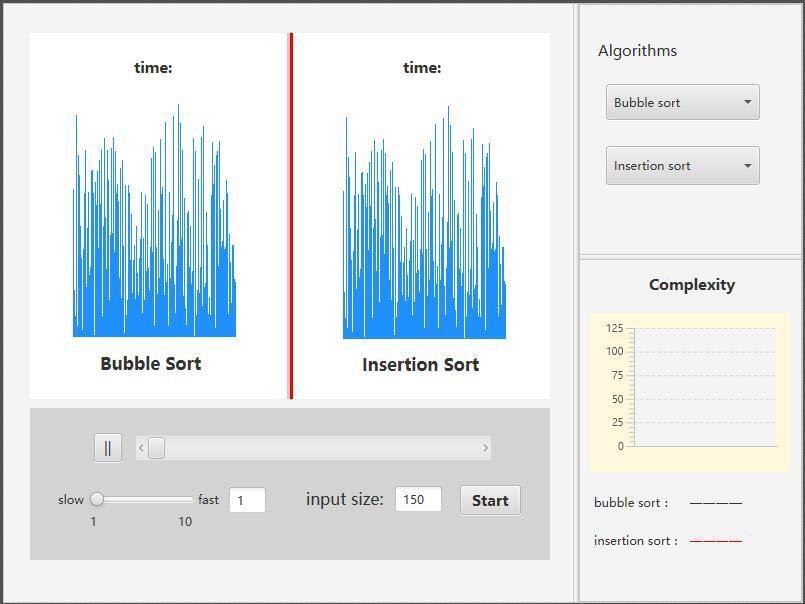
\includegraphics[width=.8\textwidth]{comparison.JPG}
\caption{comparison of the efficiency}
\label{comparison}
\end{figure}l

\begin{enumerate}
\item Selection Block\\
Comparing sorting algorithms is another function of our software. In the upper right corner of the interface, there is a selection part where users can select two algorithms to compare. After choosing the algorithms, the animation changes to two single parts which locate in left and right side. Each part is an independent part which has its own animation process. 

\item Animation\\
In each animation part, the execution time shows in the top and the name of the sorting algorithm is shown in the bottom. Below the animation, the control block is similar to the main page. Users can input the number of data in the right corner of this block.

\item Control Block\\
The control block include several buttons to control the comparing animation. For the input field, users can input the size of data so that software can generate corresponding random rectangles. When users click the start button, the two comparing frame will animate at the same time.

\item Time Complexity Block\\
Below the algorithm choosing block, there is a chart shows the time complexity of the two algorithms. After the comparing process, the chart is a clear pattern.\\

\end{enumerate}



% ------------------------------------------------------------------------------
% Implementation     
% -----------------------------------------------------------------------------
\section{Implementation}
This section introduces Implementation. Section 5.1 shows the key decisions we made and reasons. Section 5.2 describes how to implement the visualization of sorting algorithms.

\subsection{Key Implementation Decisions}

According to the Background research and user interface design, we made some key implementation decisions.
\begin{enumerate}

\item \textbf{Development Methodology}

\begin{figure}[htbp]
\centering
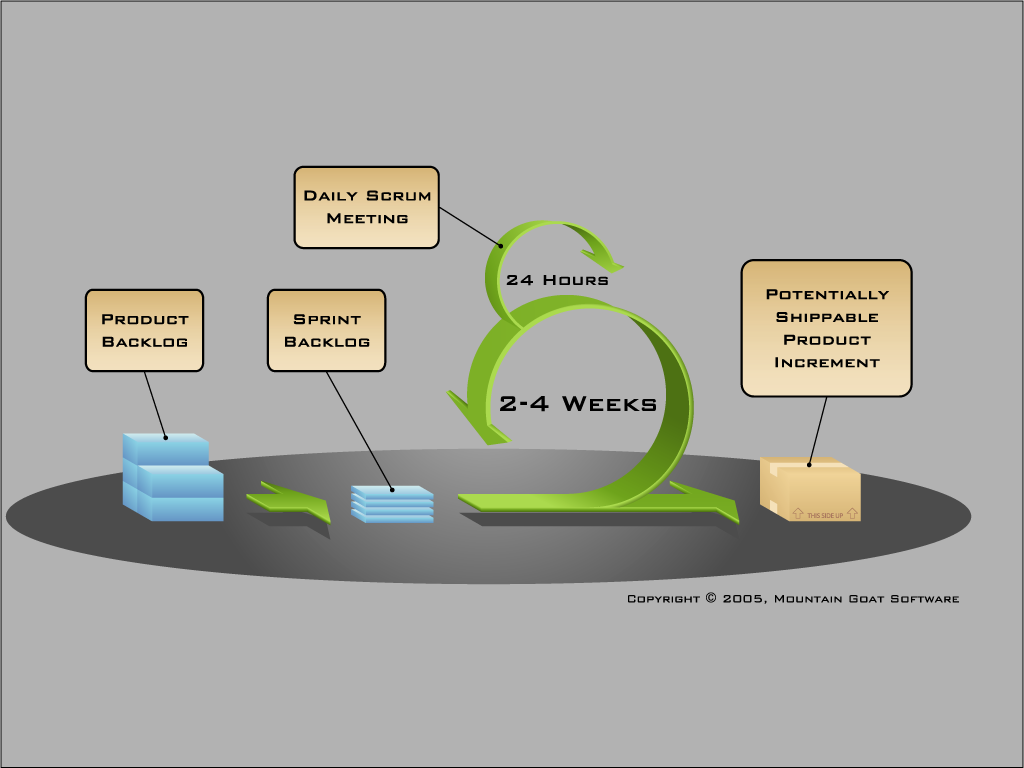
\includegraphics[width=.8\textwidth]{scrum.png}
\caption{Basic process of Scrum}
\label{scrum}
\end{figure}
	\textbf{Scrum}\\
    Scrum is an agile software development methodology, and it is an increment, iterative development process. The development process consists of a number of short iteration cycles named sprints (the green curly arrow).  The basic process of scrum\footnote{\url{https://www.mountaingoatsoftware.com/agile/scrum/overview}} is described in the Figure \ref{scrum}. In scrum, product backlog is a prioritized list of requirements used to manage product requirements. The Scrum team in a sprint should select the highest priority requirement from product backlog to develop. Then the selected requirements are analyzed and evaluated at the Scrum meeting to get a task list to be completed in the sprint called sprint backlog. When a sprint finished, the product increment is handed \cite{Scrum}. The process shows that scrum needs the team works as tight, focus on a single goal, understands the priorities and team members are clear about their roles \cite{rising2000scrum}. It is necessary for our team to work as the scrum team to develop the software. We set one sprint for a week, and finish a software requirement list as the product backlog. Our team has a short and everyday meeting to agree on a to-do-list, which will be released in a team collaboration tool named Tower as sprint backlog. In each sprint, our team will have a formal meeting with the supervisor to discuss the requirements selected and hand in product increment.
    
    \textbf{Tower}\\
Tower is an team collaboration tool which based on agile development. It can be used for Scrum to release to-do-list in each sprint. It’s like an online office where you can quickly process tasks, conduct discussions, review project progress, and work with your team at any time. According to Cockburn and Highsmith \cite{cockburn2001agile}, agile development reduces the cost of exchanging information in a team and improves the team‘s amicability—members‘ sense of community. These points are perfectly implemented in Tower. For instance, all the tasks are displayed in the panel, and team members can access all the tasks to know about the details and progress, which is easy to exchange information. Moreover, when a task is finished or assigned, every team member will be reminded, which improves the efficiency of doing tasks. It is obvious that Tower can help a lot to develop the software, so we use it as our team collaboration tool. The link is \url{https://tower.im/}.




\item \textbf{Programming languages}
The programming language is the basic part of our software. According to a website for famous programming language ranking list named TOIBE, Java is the most popular programming language in the world \cite{TIOBE2016}. Therefore, it has a huge amount of open source libraries to make our software better. Moreover, our group members are all familiar with Java. It is easier for us to develop a software. As a result, we decide to use Java as our major programming language. For the Graphical User Interface (GUI) part, we decide to use JavaFX, which is a new version GUI library for Java SE. By using JavaFX, we can also use the web language (HTML, CSS and JavaScript) indirectly to make our interface more visual.\\

\textbf{SceneBuilder JavaFX}\\
    According to Jackson, SceneBuilder JavaFX\footnote{\url{http://www.oracle.com/technetwork/java/javase/downloads/javafxscenebuilder-info-2157684.html}} provides a visual layout environment that allows us to quickly generate the main frame of the user interface for Java applications\cite{jackson2014introduction}. It supports a graphical interface control to simply drag and drop to a JavaFX scene. When one creates a user interface layout, FXML layout code will be automatically generated. SceneBuilder provides a simple and intuitive user interface that can help developers quickly create an interactive application prototype that connects GUI controls to the application logic. 
    
\textbf{External Library}\\
There is a Library for JavaFX which have some fancy and colorful components. This library is used in our user interface to help components more beautiful. jfoenix
  
\item{\textbf{Developing Tools}}\\

\textbf{IDE}\\
We decide to use eclipse. We all familiar with it. It is also convenient for us to test our code using JUnit. 


\textbf{Github}\\
According to the technical research, our group decides to use Github as a basic tool to develop the software, so that we can upload the software project to one repository where everyone can access and work on it, control the project version in case conflicts happens, and search some useful open resource distributed in Github.


\item \textbf{Platform and Operating systems}\\
For the personal computer(PC) platform, the advantage is the computer has more storage space than other devices to install an application. It also has a larger display screen, which can make animation, the main function of our software, more clear and visual. Therefore, we can design more functions for PC software development. 

For different operating system, according to StatCounter Global Stats, from 2015 to 2016, the number of users of the Windows system still possesses a high proportion of PC users \cite{Stats2016}. This situation happens not only in China, but also in the whole world. Therefore,
we realize that most of users still use the Windows system, so we decide to develop our software based on the Windows operating system. 



\end{enumerate}

\subsection{Overview of the developed source code hierarchy}





\subsection{Visualising Sorting Algorithms}

The most important part of the software is the animation of sorting algorithms. The Bubble Sort animation will be as an example to explain how we implement the animations. The basic idea of sorting algorithm animations is adding transitions to the swap function.\\

The gap of rectangles is fixed at the initial step using \texttt{HBox}.

\begin{lstlisting}
private SequentialTransition BubbleSort(int arr[], ArrayList<StackPane> list, double duration) {
        SequentialTransition sq = new SequentialTransition();
        int temp;
        for (int i = 0; i < arr.length - 1; i++) {
            for (int j = 1; j < arr.length - i; j++) {
                if (arr[j] < arr[j - 1]) {
                    temp = arr[j - 1];
                    arr[j - 1] = arr[j];
                    arr[j] = temp;
                    sq.getChildren().add(swap(list.get(j - 1), list.get(j), list, duration));
                }
            }
        }
        return sq;
    }

\end{lstlisting}

This is the function of bubble sort animation. Firstly, we use \texttt{SequentialTransition()} to make sure each action of the aniamton should act as a sequential order. The action order is added into the swap part to make rectangles move correctly. \\\\


\begin{lstlisting}
private ParallelTransition swap (StackPane l1, StackPane l2, ArrayList<StackPane> list, double speed) {
        TranslateTransition t1 = new TranslateTransition(Duration.millis(speed), l1);
        TranslateTransition t2 = new TranslateTransition(Duration.millis(speed), l2);
        ParallelTransition pl = new ParallelTransition();
        t1.setByX(30);
        t2.setByX(-30);
        pl.getChildren().addAll(t1, t2);
        Collections.swap(list, list.indexOf(l1), list.indexOf(l2));
        return pl;
    }

\end{lstlisting}

As it shown, it is \texttt{swap ()} function. Using two \texttt{TranslateTransition()} to move the recatangles which need to be swapped. 30 is the gap size of two adjacent components. Using the method \texttt{SetByX()} of \texttt{TranslateTransition ()} to set the moving distance on X-axis. Then add the two transitions into \texttt{ParallelTransition ()} to make the two swapping actions (transition) happen at the same time. 







\subsection{Implementing Graphical User Interface}

\subsubsection{Main Frame}
The “MainFrame” file designs the main interface of our software. Different components are used to implement different functions. the “menu bar” component contains different menus inside. A “Tab pane” component is used to change the pages between “Single Algorithm” and “Comparison”, which makes the page swapping more convenient and efficient. In single algorithm page, our software uses several “toggle buttons” to choose the algorithms. For each toggle button, a “ImageView” component is included to show the overview picture of the corresponding algorithm. Each button also has a “mouseEnter” function and a “mouseExit” function, which means that when the cursor move on the toggle button, the gif picture will animate, and be static if the cursor leaves. The animation block use a “hbox” component to generate the image. The progress bar and speed bar are both made by “slider” components. Both of the “initialize” button and “clear” button use “JFXbutton” components. The “play/pause” button and “random” button also use “button” components and “imageView” components inside. The input field consists of a “JFXTextField”. On the right side of the interface, two “textArea” components are used for the “Algorithm Hint block” and “Algorithm Code block”.  In comparison page, the software uses two “JFXcomboBox” to choose the algorithms, two “hbox” to show the animation and one “LineChart” component to show the complexity diagram. 
\subsubsection{Help box}
The “HelpBox” file shows the information of our software and developer. It use a “imageView” component to show our logo and a button “ok” to confirm and quit the dialog. Other word information is included in the “Text” component. 
\subsubsection{Preference}
The “Preference” file shows the interface of color choosing function. It uses a “JFXColorPicker” component to choose the color for generated image and a button “Apply” to confirm and quit the dialog.
\subsubsection{Guideline}
The “Guideline” file designs the guide page of our software. It uses a “TabPane” component to change the guide pages between “Single Algorithm” and “Comparison”. It also has a button “ok” to confirm and quit the dialog.
\subsubsection{Menu bar}
In this section, two important functions in menu bar will be introduced, the first one is "Save Code" function in "File" menu, and the second one is "Code Language" function in "Function" menu.
\begin{itemize}
\item "Save Code" function
\item "Code Language" function
\end{itemize}









% ------------------------------------------------------------------------------
% Test (1000)----Yangyu Gao
% -----------------------------------------------------------------------------
\section{Testing}
% ------------------------------------------------------------------------------
%Achieved work with requirements (600)
%Summary of what was achieved, referring to the stated requirements.
% ------------------------------------------------------------------------------
In this chapter, the testing of the application will be involved. For all the function requirements, we test them by using Black Box Testing. In addition, the User Interface Testing is used to test the user interface (UI)  of the software. Otherwise, the future works are shown in the following part, which include the introduction of the incomplete functions and the functions that can be achieved in the future.

\subsection{Black Box Testing}
To check whether the application has correspond with the functional requirement, the black box testing has been used. Black box testing is a testing way which only examines application's functionality, it does not peer into the internal part of the application otherwise. By doing the black box testing, the following errors could be found: \\
\begin{itemize}
\item Incorrect or missing functions
\item Interface errors
\item Initialization and termination errors
\end{itemize}
The table below shows the test process and the result of this application's black box testing.

% table
\begin{table}[H]
\begin{tabular}{|p{4cm}|p{4cm}|p{5cm}|p{0.5cm}|}
\hline
\multicolumn{4}{|c|}{System Test Sheet} \\ \hline
\multicolumn{1}{|c|}{Project Title} & \multicolumn{3}{l|}{AlgoDomino} \\ \hline
\multicolumn{1}{|c|}{Objective} & \multicolumn{3}{l|}{To test whether the system meets the functional requirements.} \\ \hline
\multicolumn{1}{|c|}{Method} & \multicolumn{3}{l|}{Black Box Testing} \\ \hline
\multicolumn{1}{|c|}{Test Environment} & \multicolumn{3}{l|}{} \\ \hline
\multicolumn{4}{|c|}{Test Progress} \\ \hline
\multicolumn{1}{|c|}{Requirement to the test} & \multicolumn{1}{c|}{Action} & \multicolumn{1}{c|}{Expected Result} & \multicolumn{1}{c|}{Y/N} \\ \hline
The software should provide users a guide of how to use core features. & Help - Domino Help & A window pops up which shows the guide of this software & Y \\ \hline
The software should allow users to select which sorting algorithms to animate. & Click Single Algorithm (under the menu bar)- Click the sort button & After clicking, the button generates a blue border, and the background color changed & Y \\ \hline
The software should be able to allow users to define input data by themselves. & Input a sequence of integers following the provided format & The text area shows what user has input & Y \\ \hline
 & Click CLEAR button & Empty the input area & Y \\ \hline
The software should be able to generate input data randomly. & Click RANDOM button (represent by a "dice") & A sequence of numbers appear in the input text area & Y \\ \hline
The software should be able to visualize the processes of running a sorting algorithm. & Click INITIALIZE button & The animation board generates a sequence of rectangles with text of numbers, which the rectangles' height and the numbers are connected with the input & Y \\ \hline
The software should allow users to start, stop, slow down, speed up, restart or pickup a point of the animation. & Click START/PAUSE button & Animation starts to run, the START/PAUSE button change to from START to PAUSE, the input area cannot input integers at this moment, the time slider start to move & Y \\ \hline
& Click START/PAUSE button & Animation paused, the START/PAUSE button change from PAUSE to START, the time slider stop to move & Y \\ \hline
\end{tabular}
\end{table}

\begin{table}[H]
\begin{tabular}{|p{4cm}|p{4cm}|p{5cm}|p{0.5cm}|}
\hline
 & Drag SPEED SLIDER to change the speed of the animation & The speed of the animation changed & Y \\ \hline
 & Drag TIME SLIDER to change & The animation changed & Y \\ \hline
 & Click NEXT STEP button (left side of the START/PAUSE button) & The animation moves to next movement & N \\ \hline
 & Click LAST STEP button (right side of the START/PAUSE button) & The animation moves to previous movement & N \\ \hline
The software should be able to show the running sorting algorithm's source Javacode to users. & Click START/PAUSE button & The code shows on the Algorithm Code part, which is in the right part of the interface & Y \\ \hline
The software should be able to match specific line of running sorting algorithm's source code and its explanation with animation. & Click START/PAUSE button & In the Algorithm Code part, the specific line of code is highlighted & N \\ \hline
 &  & In the Algorithm Hint part (above the Algorithm Code part), the explanation of the sorting algorithm appeared & Y \\ \hline
The software should allow users to select which algorithms to compare. & Click Comparison button (between the Single Algorithm button) - Click to choose two algorithms (right side of the interface) & Two algorithms has been chosen, two labels show the name of the algorithms on the animation window and complexity window (under the algorithm choosing part) & Y \\ \hline
The software should compare the efficiency of different sorting algorithms by showing the animation simultaneously. & Input a range of integers following the input area's default format - Click START button & The animation window generates two groups of rectangles and start to run different animations depends on what user choose & Y \\ \hline
 &  & The algorithm's running time will be shown under each single animation window & Y \\ \hline
\end{tabular}
\end{table}
 
\begin{table}[H]
\begin{tabular}{|p{4cm}|p{4cm}|p{5cm}|p{0.5cm}|}
\hline
The software should be able to provide the time complexities of sorting algorithms when comparing the efficiency. & Click START button & A chart will be shown in the Complexity window (right part of the main interface) according to the times of these two algorithms & Y \\ \hline
The software should allow users to customize the interface, such as the background color of animation, shapes and colors of basic components used in an animation. & Click Function button - Click Color of Chart - Select a color - Click Apply button & The color of rectangles are changed & Y \\ \hline
Users should be able to download the source code of selected sorting algorithms in several programming languages. & Click File button on the top bar-Click Save Code & Save the code of the algorithm & Y \\ \hline
Users should be able to save the screen-shot of the current interface & Click File button - Click Save Screen-Shoot & Save the algorithm animation as screen-shot & Y \\ \hline
\end{tabular}
\end{table}

\subsection{Evaluation and Discussion}

\subsubsection{User Interface Testing}
Because the black box test can not test the functions without code, so we need to change the way of testing the GUI part.\\
\newline
When open the software, the screen of the software is validate, nothing lost and miss. For the navigation, all the button have a react after clicking it. When input something in the input area, the text area shows the input smoothly. When using the software, all the manipulations are reacting without delay.


\subsubsection{Future Work}
To enhance the usability of the software, there are also some things we would like to do. Firstly, the User Interface (UI) design have lifting space. We make the window of the software as fixed size, it can be improved to resizable, and the inner windows' size will also be changed automatically. In addition, the shape of components of animation need to be changed by users in the future, which can fit the user center model and make users feel more comfortable to see the animation.\\
\newline
In terms of skill improvement, we want increase the number of algorithms for the animation part which means people can learn more algorithms from our software. Moreover, the highlight of the code which need to synchronize with the sort animation is not achieved because of the limitation of the language. If there are some technical to solve it ,it is better for user to learn.\\
\newline
Finally, it is more convenient for users to have multiple platforms to operate the system. People can learn sorting algorithms everywhere by smart phone or pad.



% ------------------------------------------------------------------------------
% Reflective Comments
% -----------------------------------------------------------------------------
\section{Reflective Comments}
\subsection{Time line}\\
\subsection{Problems Encountered and Solutions}
\begin{enumerate}
	\item \textbf{Technical problem}\\
Since this is the first time we try to develop a software, we lack of some vital skills for this project. Therefore, we try to find some upperclassmen to ask how to plan our project. Then we find the agile development method is suitable for us. Based on this method, we have an appropriate plan of the project. \\

In addition, we do not learn GUI before. It is difficult for us to make animations. We choose JavaFx as our main language. However, there is little tutorial of JavaFx. It is very hard for us to code at the first stage. Then we are more familiar with this language by checking API and learning from other people. 

    \item \textbf{Group roles}\\
As a new team builds up, we do not know each other. It is difficult for team leader to know teammates' strengths and weaknesses in a short time. Thus we do not have a clear group role for everyone originally, and it causes some trouble in assigning tasks. At the third week of the first semester, we distributed our roles of the project. It is very useful for us to distribute tasks. 


    \item \textbf{Task overdue}\\
Sometimes tasks were overdue by some reasons, and it delays the progress of the project. Therefore, to prevent this problem, we try to use a team-collaboration software named tower to manage and distribute our tasks. It can record tasks, their implementers and due days. If someone does not finish the task in time, it would remind us. It is extremely efficient to solve this problem. Our members can get motivated by this method.

    \item \textbf{Missing stakeholders}\\
Our project does not have any stakeholders; we need to figure out all requirements by ourselves. To make the requirements clearer, we find some people to ask for suggestions. The supervisor also give us many useful suggestions based on her experience.

	\item \textbf{ Inappropriate Time Schedule}\\
It is very difficult to make a perfect plan. Although we plan for our project, some problems break the plan. Firstly, there are some function we cannot achieve in time. It is very time-consuming to fix bugs. secondly, at the former stage, we do not concentrate on the most important part. We try to add more functions for the software, but ignore to make the better quality of animations. 

\end{enumerate}

\subsection{What we have learnt}
Firstly, it is very happy to have the chance to work with group. We have learnt how to do a project more efficiently. We are more familiar with the process of software engineering. It is a good experience for future projects. We also know how to use tools to help us such as using github to track code.\\

Secondly, the skill of coding is increasing. Although we all did not use JavaFX before, we can use it make a software in a short time. It is very amazing based on our level because we did not have the experience to work with a software engineering project before.\\

Thirdly, we know the importance of collaboration. If the team members do not help each other, we will not finish the project. Our members are all pleased to share their knowledge to help each other.\\












% ------------------------------------------------------------------------------
% Conclusion
% -----------------------------------------------------------------------------
\section{Conclusion}
Overall, we think the project was a success, as it solves the problem asked and meets all the main requirements.

The project had originally aimed to implement the functionality for the user to be able to change shapes of animation and more interesting functions, however as the project went on, it became ever more apparent how hard this feature would be to implement and the time is limited, instead of half-implementing it, it was decided to focus on making the basic features of the system stronger. 

In summary, this project achieved the aims that we were required. We believe that the software can help students study the sorting algorithms easier.


% ------------------------------------------------------------------------------
% Appendix
% -----------------------------------------------------------------------------
\section{Appendix}

\subsection{Description of Testing}
\subsection{Meeting Minutes}
------------------------------------------------------------------------------------\\
\textbf{Meeting: 26 Sep. 2016}\\


Student: Zhefeng ZHOU, Yangyu GAO, Muyi JIANG, Jiaying SUN, Kan LIU, Zhe REN\\
Supervisors: Heshan DU\\

\textbf{Aim:} \\
To discuss how to have a head start of our project.\\

\textbf{Agenda:} \\
1.	Background research\\
2.	Java GUI programming\\
3.	Algorithm in prototype\\\\

\textbf{Discussion}:\\
1.	Background search\\

We discussed two ways to do background search, one is issuing questionnaire and other one is searching similar apps via Internet and checking their features.\\
 
2.	Java GUI tutorial\\

We discussed how to make a head start of Java GUI programming, and decided to start from the textbook and produce simple demo to get familiar with related packages.\\
   
3.	Algorithm in prototype\\

We discussed which sorting algorithm to start with when developing the prototype.  Possible options include bubble sort, selection sort and insertion sort, we’ll learn a little bit and discuss it before 30 Sep. 2016.\\\\

\textbf{Action Points}\\
1.	Set up the website for the project\\
2.	Design and issue the questionnaire, and send a draft to Heshan\\
3.	Start to prepare the first version of requirement specification\\
4.	Produce simple java programs with GUI\\
5.	Decide which algorithm would be used in the prototype, learn and implement it in java code\\
6.	Start to learn Latex, get the software download and installed on the computer\\

\textbf{Next Meeting: 10 Oct. 2016}\\
------------------------------------------------------------------------------------\\
\textbf{Meeting: 10 Oct. 2016}\\


Student: Zhefeng ZHOU, Yangyu GAO, Muyi JIANG, Jiaying SUN, Kan LIU, Zhe REN\\
Supervisors: Heshan DU\\

\textbf{Aim:} \\
To discuss methods to specify our jobs of this project.\\

\textbf{Agenda:} \\
1.	Website template\\
2.	Draft of questionnaire\\
3.	Requirement specification\\
4.	Report\\\\

\textbf{Discussion}:\\
1.	Website template\\

We planed to use a web page template to create our website. This template 		   contains a timeline as a clue, which is convenient to record the progress of our project.\\
 
2.	Draft of questionnaire\\

Firstly, we discussed the context of the questionnaire template. Some questions of it are not suitable, so we decided to make questions more specific and focus on smaller group like classmates.  \\
	Then, we discussed research checklist. There are some problems need to be revised, such as the relevance of secondary data sets. In addition, we knew there is some jobs of making a questionnaire, such as attaching information sheet and assigning identified id number, etc.\\

   
3.	Requirement specification\\

We discussed which sorting algorithm to start with when developing the prototype.  Possible options include bubble sort, selection sort and insertion sort, we’ll learn a little bit and discuss it before 30 Sep. 2016.

4.	Report\\

We discussed that when we should start to write interim report. We decided to 	accomplish a draft of interim report two weeks earlier than the deadline to have enough time to revise.\\\\

\textbf{Action Points}\\
1.	Prepare website\\
2.	Try to solve the problems of questionnaire\\
3.	Prepare draft of requirement specification\\
4.	Keep learning Java GUI programming and LaTex\\
5.	Consider the date of writing report\\
	 
\textbf{Next Meeting: 17 Oct. 2016}\\
------------------------------------------------------------------------------------\\
\textbf{Meeting: 17 Oct. 2016}\\


Student: Zhefeng ZHOU, Yangyu GAO, Muyi JIANG, Jiaying SUN, Kan LIU, Zhe REN\\
Supervisors: Heshan DU\\

\textbf{Aim:} \\
To discuss methods to specify our jobs of this project.\\

\textbf{Agenda:} \\
1.	Website fix\\
2.	Questionnaire cancelation\\
3.	Requirement specification\\
4.	Software platform\\
5.	Dissertation view\\\\

\textbf{Discussion}:\\
1.	Website fix\\

We finished our website page temple and there remained some small changes to be made. We would complete it before the next formal meeting.\\

 
2.	Questionnaire cancelation\\

We decided to cancel the questionnaire due to the fact that it’s not suitable for our project.\\


   
3.	Requirement specification\\

We viewed part of the first version of our requirement specification. Some details would be added and changes would be made during our software development process.\\


4.	Software platform\\

We haven’t decided which platform to show our software on and we discussed previous year students’ choices of software platforms. Most of them chose windows only. The decision would be made after our group meeting this week.\\

5.	Dissertation view\\

We picked and scanned some dissertations that are helpful for the preparation of our report. \\\\

\textbf{Action Points}\\
1.	Make some changes of our website\\
2.	Accomplish requirement specification as the project develops\\
3.	Decide the platform of project and prepare for it.\\
4.	Study the related dissertation and prepare for our report.\\
5.	Keep learning Java GUI programming and LaTex\\

\textbf{Next Meeting: 24 Oct. 2016}\\
------------------------------------------------------------------------------------\\
\textbf{Meeting: Meeting: 7 Nov. 2016}\\


Student: Zhefeng ZHOU, Yangyu GAO, Muyi JIANG, Jiaying SUN, Kan LIU, Zhe REN\\
Supervisors: Heshan DU\\

\textbf{Aim:} \\
To discuss methods to specify our jobs of this project.\\

\textbf{Agenda:} \\
1.	Requirement Specification V3\\
2.	Website design\\
3.	GUI design\\
4.	Suggestion on system architecture\\\\


\textbf{Discussion}:\\
1.	Requirement Specification V3\\

	We decided to modify the Introduction part to make the requirement specification fit in interim report.\\
	We decided to make some user stories and UML design, then put them in a motivation part in interim report rather than requirement specification part.\\
    
2.	Website design\\

	We decided to improve the home page of website in the following two parts\\
1)	The homepage should introduce the software and its main function.
2)	The homepage should explain why our group is called “Grape”.
	We decided that the function of comment is not necessary.

3.	GUI design\\

	We decided to improve the mainframe part\\
1)	The choosing algorithm button should show the full name of sort algorithm.
2)	The input box should prompt users the format of input.
3)	The progress bar should be under the bar graph.
4)	We will decide where to put the “Random generate” button.\\\\
	We decided to improve the comparison part \\
1)	We will reduce the number of choosing algorithm button to 2.
2)	We will show the complexity of two algorithms in one coordinate system.
3)	We will consider how to design the “Stop” button.
4)	We will consider the relation between input size and complexity in coordinate system.\\


4.	Suggestion on system architecture\\

	We decided to focus on one algorithm and try to implement its main function. \\\\

\textbf{Action Points}\\
1.	Improve requirement specification\\
2.	Improve website homepage\\
3.	Improve GUI design\\
4.	Prepare the interim report\\
5.	Learn the user interaction model\\
6.	Make some user stories and UML design\\


\textbf{Next Meeting: 14 Nov. 2016}\\
------------------------------------------------------------------------------------\\

\subsection{Sorting Algorithms Pseudocode}
\renewcommand{\algorithmicrequire}{\textbf{Input:}}
\renewcommand{\algorithmicensure}{\textbf{Output:}}
    \begin{algorithm}
        \caption{Bubble Sort}
        \begin{algorithmic}[1] 
            \Require $Array,size$
            \Ensure Sorted array
            \Function {bubbleSort}{$Array, size$}
                \State $i \gets 0$
                \State $j \gets 0$
                \For{$i = 0 \to size-1$}
                 \For{$j = 0 \to size-1-i$}
                    \If {$Array[j] < array[j+1]$}             
                    \State \Call{swap}{$Array[j],Array[j+1]$}
                    \EndIf
                  \EndFor
                \EndFor
            \EndFunction
        \end{algorithmic}
    \end{algorithm}

\renewcommand{\algorithmicrequire}{\textbf{Input:}}
\renewcommand{\algorithmicensure}{\textbf{Output:}}
    \begin{algorithm}
        \caption{Insertion Sort}
        \begin{algorithmic}[1] 
            \Require $Array,size$
            \Ensure Sorted array
            \Function {nsertionSort}{$Array, size$}
                \For{$i = 1 \to size$}
                 \State $j \gets i$
                 \While{$j>0$ \textbf{and} $Array[j-1]>Array[j]$}
                \State \Call{swap}{$Array[j],Array[j-1]$}
                \State $j \gets j-1$
                \EndWhile
                \EndFor
            \EndFunction
        \end{algorithmic}
    \end{algorithm}
    
\renewcommand{\algorithmicrequire}{\textbf{Input:}}
\renewcommand{\algorithmicensure}{\textbf{Output:}}
    \begin{algorithm}
        \caption{Selection Sort}
        \begin{algorithmic}[1] 
            \Require $Array,size$
            \Ensure Sorted array
            \Function {selectionSort}{$Array, size$}
                \For{$i = 0 \to size-1$}
                 \State $index \gets i$
                 \For{$j = i+1 \to size$}
                    \If{$Array[index]>Array[j]$}
                 	\State $index \gets j$
                 \EndIf
                \EndFor
                 \State \Call{swap}{$Array[index],Array[i]$}
                \EndFor
            \EndFunction
        \end{algorithmic}
    \end{algorithm}
    
\renewcommand{\algorithmicrequire}{\textbf{Input:}}
\renewcommand{\algorithmicensure}{\textbf{Output:}}
    \begin{algorithm}
        \caption{Quick Sort}
        \begin{algorithmic}[1] 
            \Require $Array,size$
            \Ensure Sorted array
            \Function {quickSort}{$Array, size$}
            \State $ var\ lessList, pivotList, greaterList$
             \If{$size<=1$}
                 \State \Return{$Array$}
             \Else
             \State $select\ a\ pivot\ value\ pivot\ \ q$
             \For{$each\ x\ in\ q\ except\ the\ pivot\ element$}
                \If{$x<pivot$}
                 \State $add\ x\ to\ lessList$
                 \EndIf
                 \If{$x>=pivot$}
                 \State $add\ x\ to\ greaterList$
                 \EndIf
              \State $ add\ pivot\ to\ pivotList$
             \EndFor
            \State \Return {$concatenate(QUICKSORT(lessList),pivotList,QUICKSORT(greaterList))$}
           \EndIf
            \EndFunction
        \end{algorithmic}
    \end{algorithm}
    
\renewcommand{\algorithmicrequire}{\textbf{Input:}}
\renewcommand{\algorithmicensure}{\textbf{Output:}}
    \begin{algorithm}
        \caption{Merge Sort}
        \begin{algorithmic}[1]
            \Require $Array,n$
            \Ensure Sorted array
            \Function {mergeSort}{$Array, left, right$}
                \State $result \gets 0$
                \If {$left < right$}
                    \State $middle \gets (left + right) / 2$
                    \State $result \gets result +$ \Call{Merge Sort}{$Array, left, middle$}
                    \State $result \gets result +$ \Call{Merge Sort}{$Array, middle, right$}
                    \State $result \gets result +$ \Call{Merger}{$Array,left,middle,right$}
                \EndIf
                \State \Return{$result$}
            \EndFunction
            \State
            \Function{Merger}{$Array, left, middle, right$}
                \State $i\gets left$
                \State $j\gets middle$
                \State $k\gets 0$
                \State $result \gets 0$
                \While{$i<middle$ \textbf{and} $j<right$}
                    \If{$Array[i]<Array[j]$}
                        \State $B[k++]\gets Array[i++]$
                    \Else
                        \State $B[k++] \gets Array[j++]$
                        \State $result \gets result + (middle - i)$
                    \EndIf
                \EndWhile
                \While{$i<middle$}
                    \State $B[k++] \gets Array[i++]$
                \EndWhile
                \While{$j<right$}
                    \State $B[k++] \gets Array[j++]$
                \EndWhile
                \For{$i = 0 \to k-1$}
                    \State $Array[left + i] \gets B[i]$
                \EndFor
                \State \Return{$result$}
            \EndFunction
        \end{algorithmic}
    \end{algorithm}
    
\renewcommand{\algorithmicrequire}{\textbf{Input:}}
\renewcommand{\algorithmicensure}{\textbf{Output:}}
    \begin{algorithm}
        \caption{Heap Sort}
        \begin{algorithmic}[1] 
            \Require $Array,size$
            \Ensure Sorted array
            \Function {heapSort}{$Array, size$}
               \For{$i = size/2 \to 0$}
                   \State \Call{HEAPIFY}{$Array,i,size-1]$}
                \EndFor
                 \For{$i = size-1 \to 1$}
                   \State \Call{Swap}{$Array[i],Array[0]]$}
                   	\State \Call{HEAPIFY}{$Array,0,i]$}
                \EndFor
            \EndFunction
            \State
            \Function{HEAPIFY}{$Array, parrent, size$}
                \State $temp \gets Array[parent]$
                \State $child\gets 2*parent+1$
                \While{$child<size$}
              \If{$child+1<length$ \textbf{and} $Array[child]<Array[child+1]$}
      				\State $child \gets child+1$
              \EndIf
              \If{$temp>=Array[child]$}
      					\State $break$
               \EndIf
                \State $Array[parent] \gets Array[child]$
                \State $parent\gets child$
                \State $child\gets 2*child+1$
                \EndWhile
                \State $Array[parent] \gets temp$
            \EndFunction
        \end{algorithmic}
    \end{algorithm}

\subsection{User Manual}
\begin{figure}[htbp]
\centering
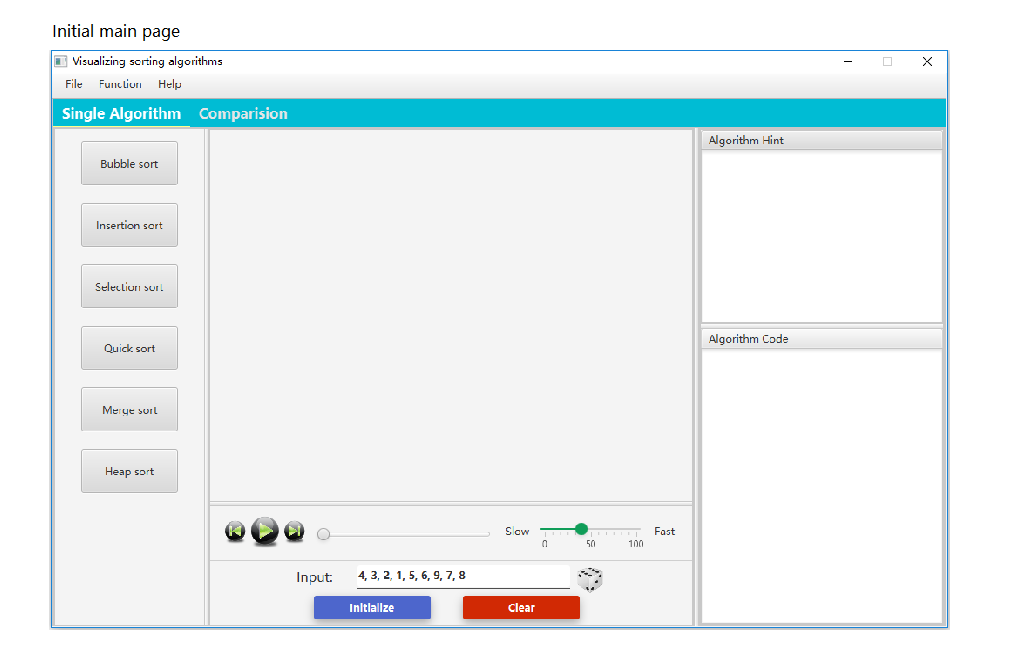
\includegraphics[width=1\textwidth]{user_menu/1.png}
\label{user_menu1}
\end{figure}

\begin{figure}[htbp]
\centering
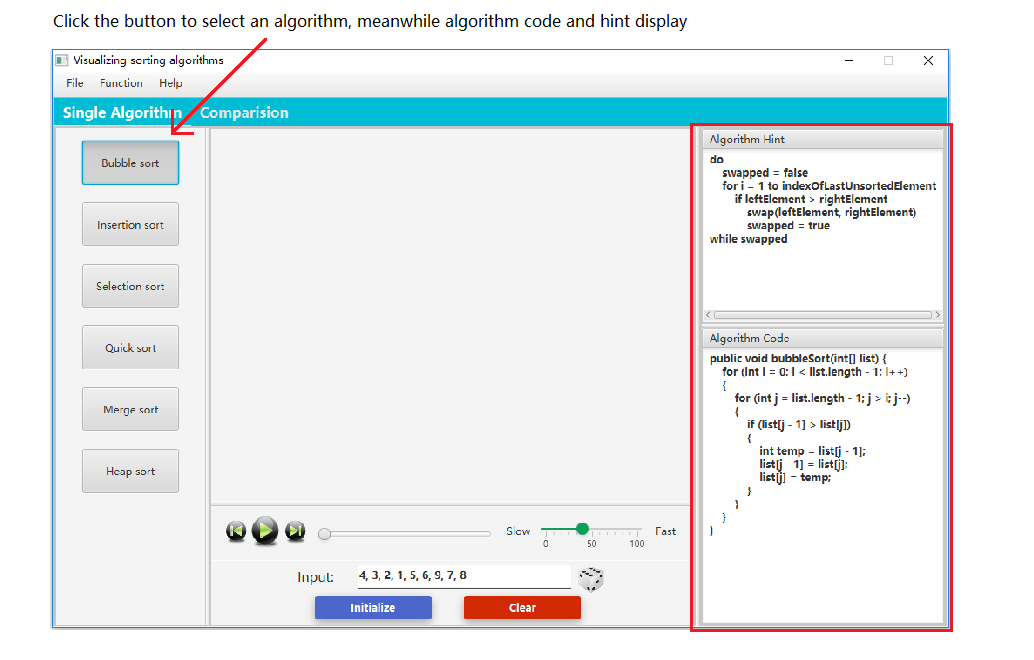
\includegraphics[width=1\textwidth]{user_menu/2.png}
\label{user_menu2}
\end{figure}

\begin{figure}[htbp]
\centering
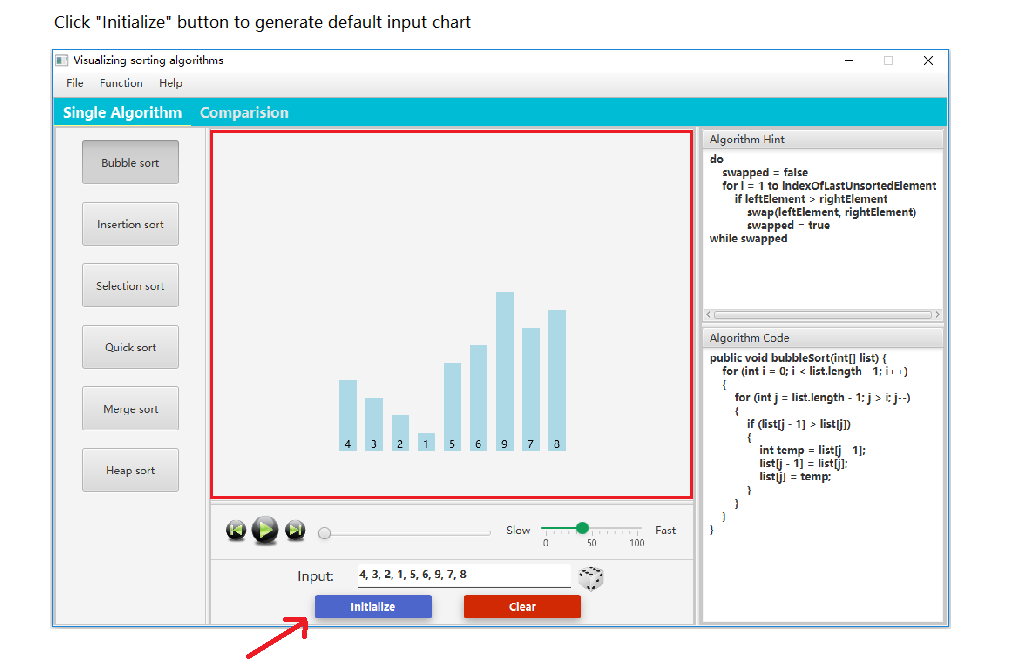
\includegraphics[width=1\textwidth]{user_menu/3.png}
\label{user_menu3}
\end{figure}

\begin{figure}[htbp]
\centering
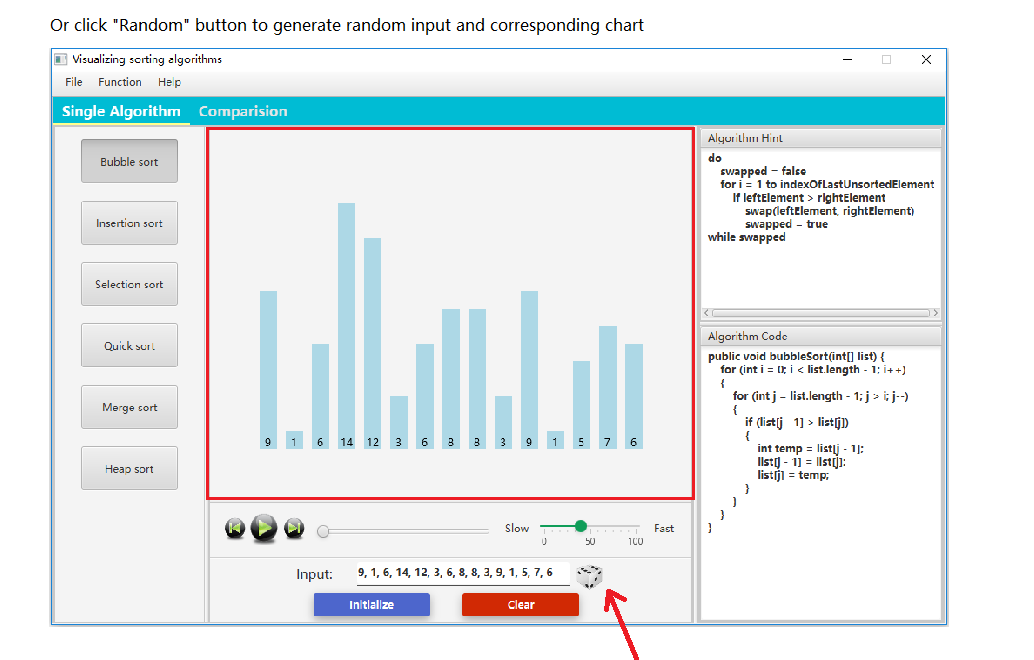
\includegraphics[width=1\textwidth]{user_menu/4.png}
\label{user_menu4}
\end{figure}

\begin{figure}[htbp]
\centering
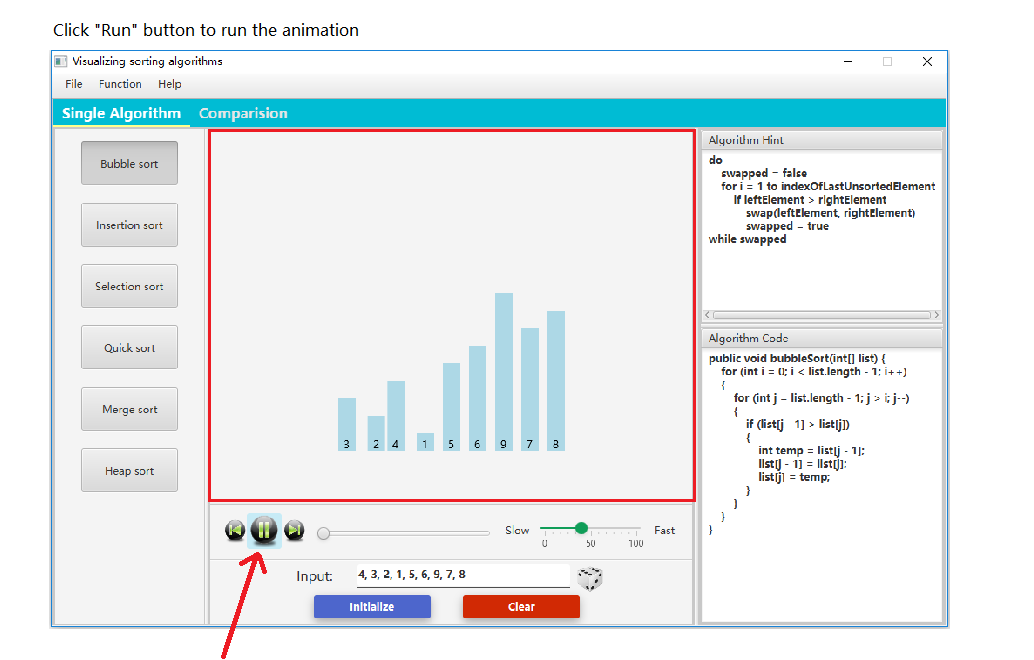
\includegraphics[width=1\textwidth]{user_menu/5.png}
\label{user_menu5}
\end{figure}

\begin{figure}[htbp]
\centering
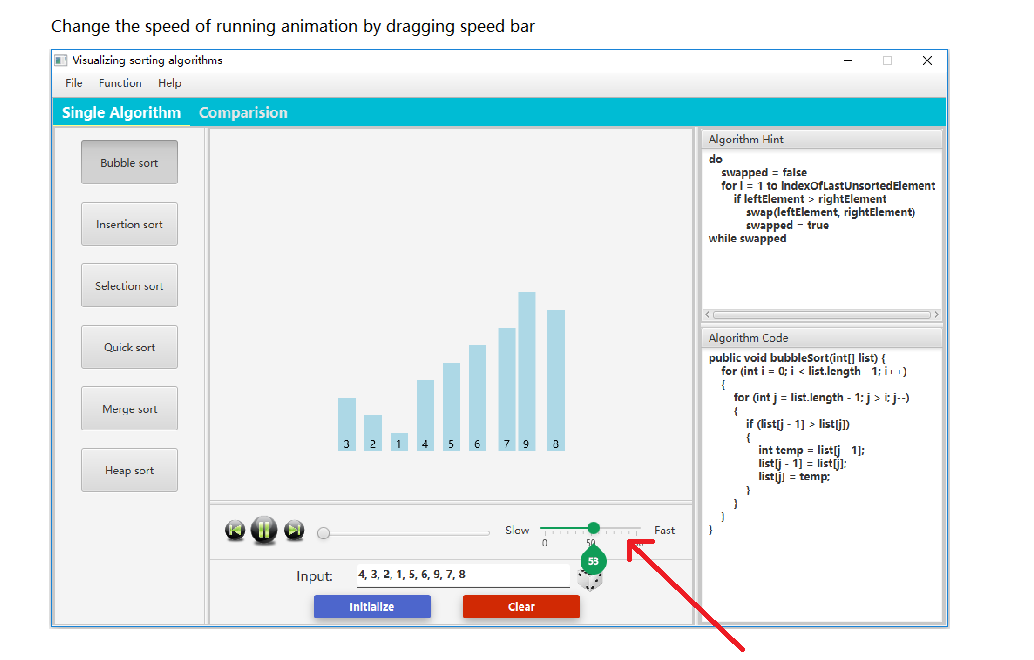
\includegraphics[width=1\textwidth]{user_menu/6.png}
\label{user_menu6}
\end{figure}

\begin{figure}[htbp]
\centering
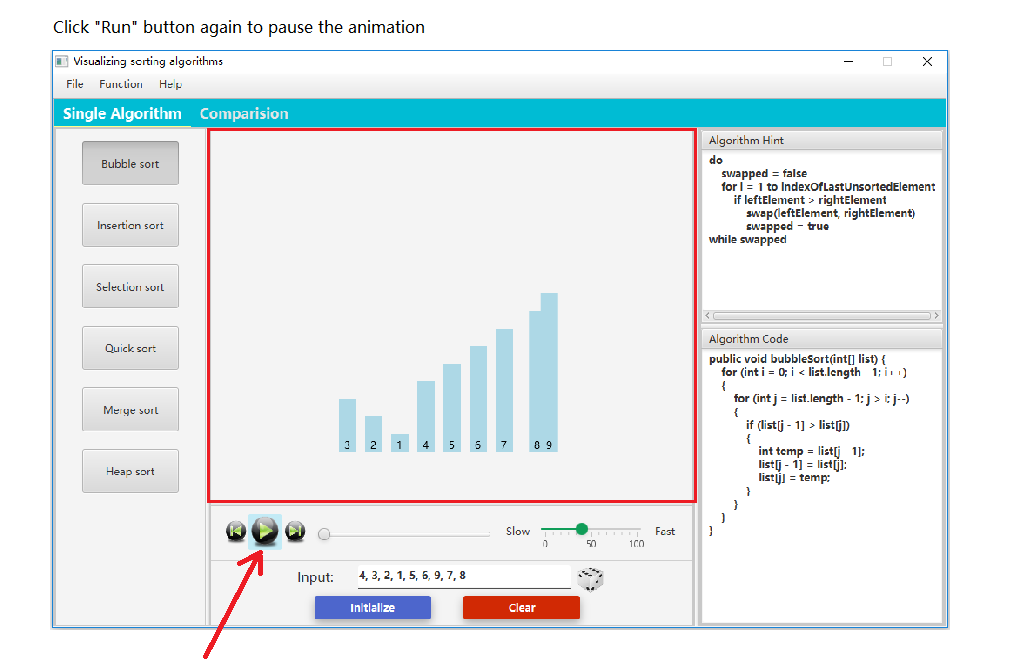
\includegraphics[width=1\textwidth]{user_menu/7.png}
\label{user_menu7}
\end{figure}

\begin{figure}[htbp]
\centering
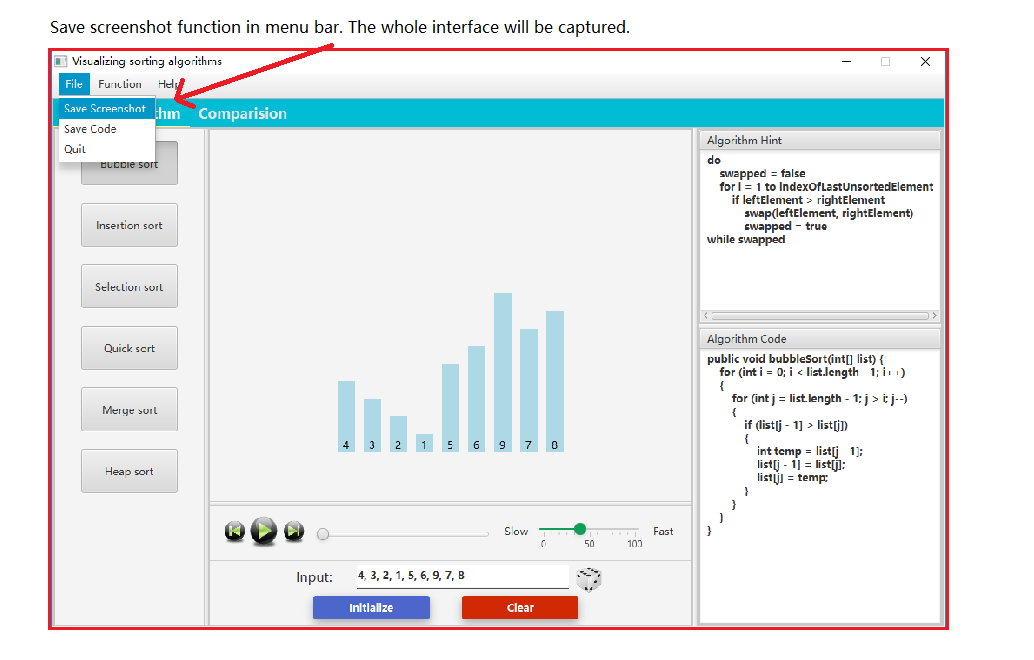
\includegraphics[width=1\textwidth]{user_menu/8.png}
\label{user_menu8}
\end{figure}

\begin{figure}[htbp]
\centering
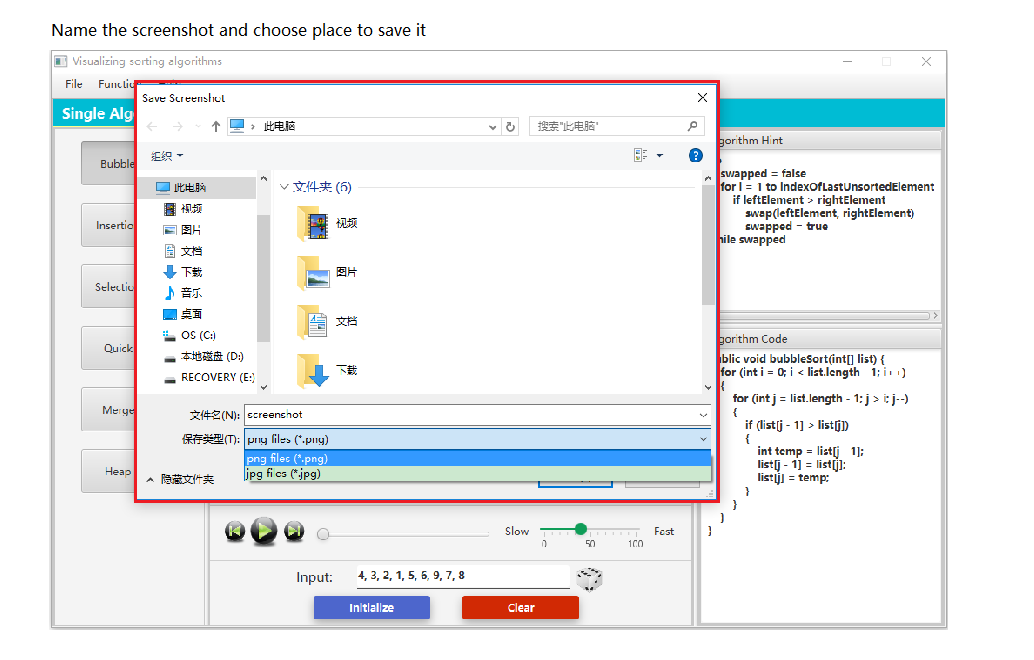
\includegraphics[width=1\textwidth]{user_menu/9.png}
\label{user_menu9}
\end{figure}

\begin{figure}[htbp]
\centering
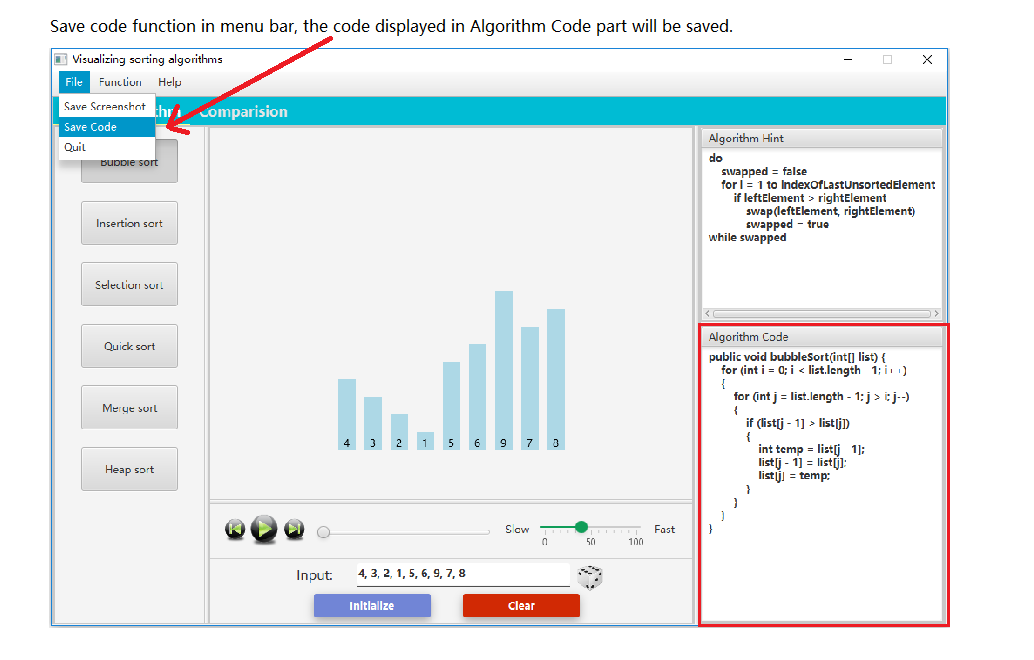
\includegraphics[width=1\textwidth]{user_menu/10.png}
\label{user_menu10}
\end{figure}

\begin{figure}[htbp]
\centering
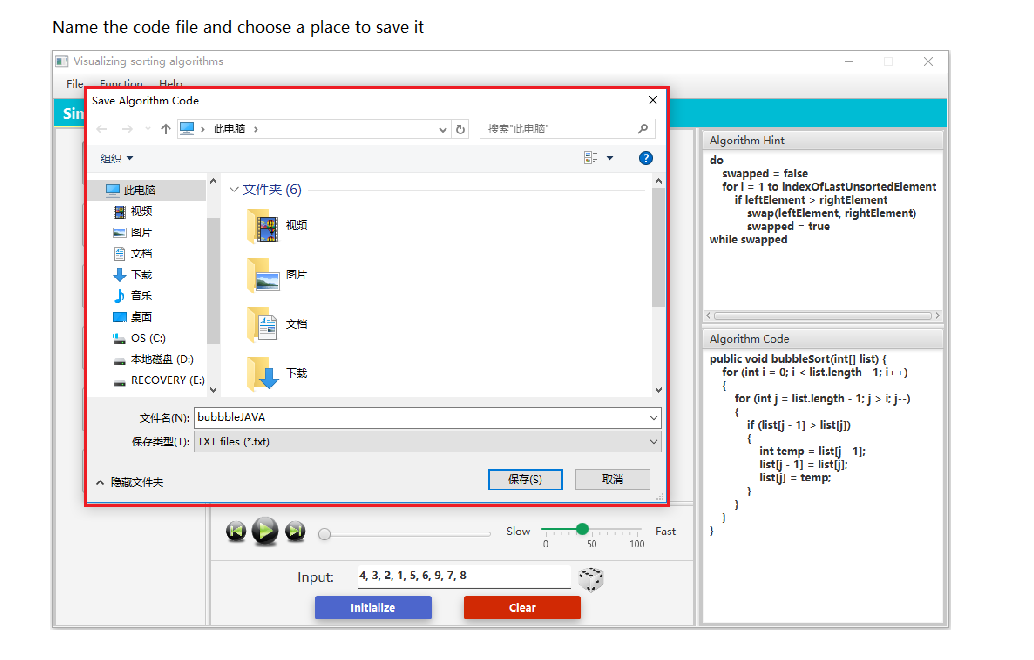
\includegraphics[width=1\textwidth]{user_menu/11.png}
\label{user_menu11}
\end{figure}

\begin{figure}[htbp]
\centering
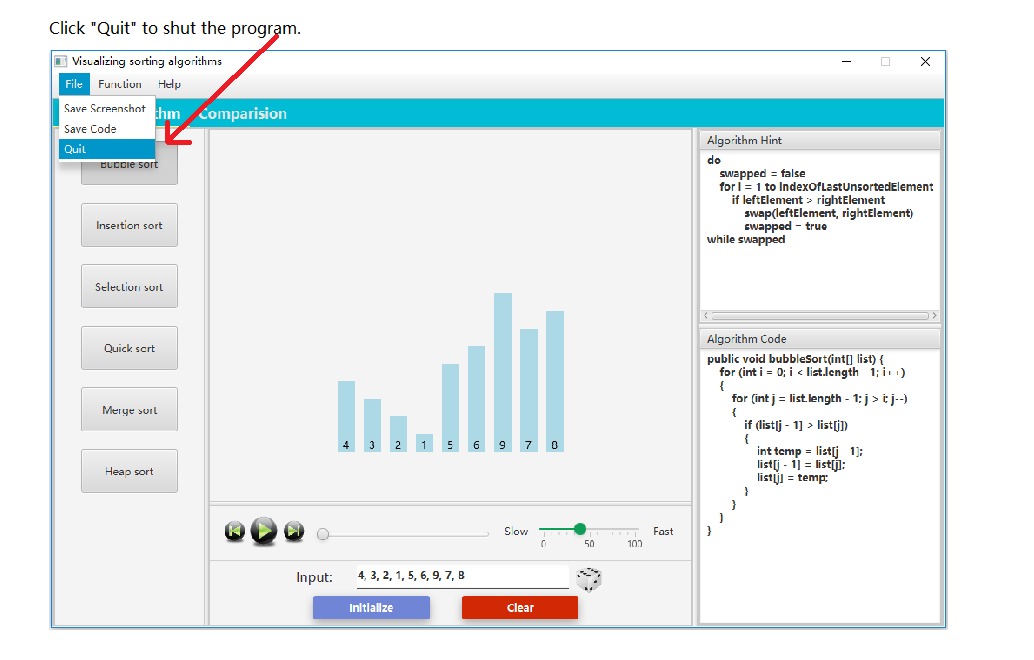
\includegraphics[width=1\textwidth]{user_menu/12.png}
\label{user_menu12}
\end{figure}

\begin{figure}[htbp]
\centering
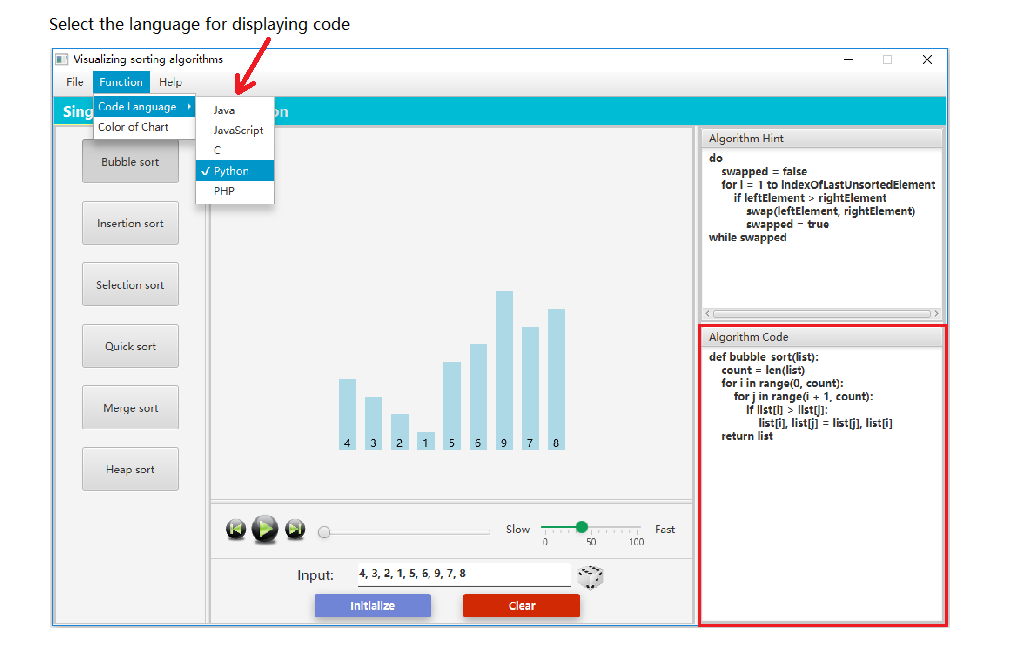
\includegraphics[width=1\textwidth]{user_menu/13.png}
\label{user_menu13}
\end{figure}

\begin{figure}[htbp]
\centering
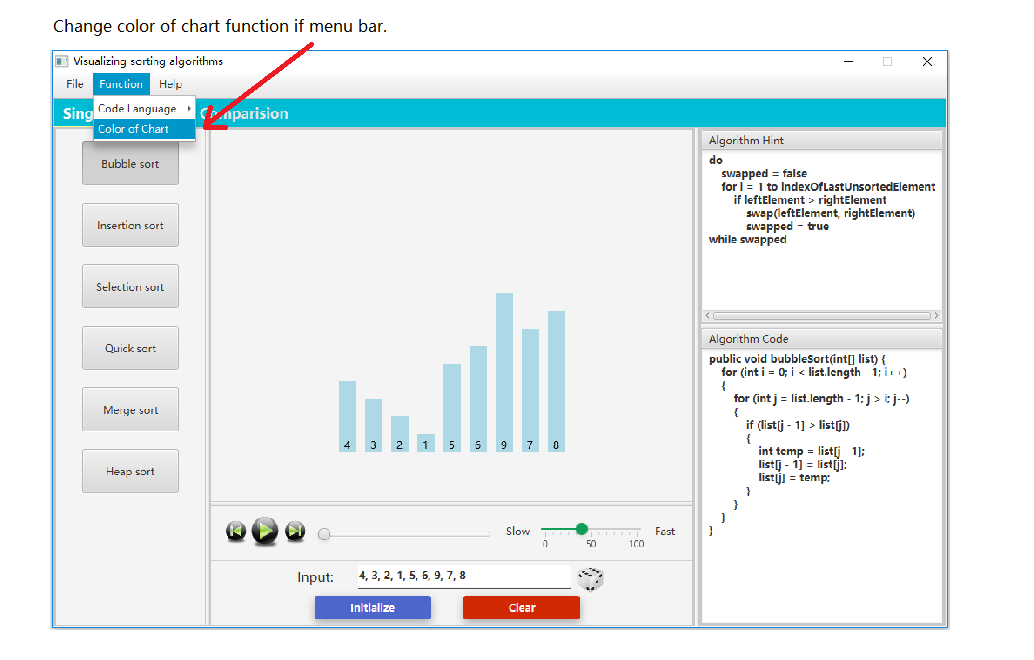
\includegraphics[width=1\textwidth]{user_menu/14.png}
\label{user_menu14}
\end{figure}

\begin{figure}[htbp]
\centering
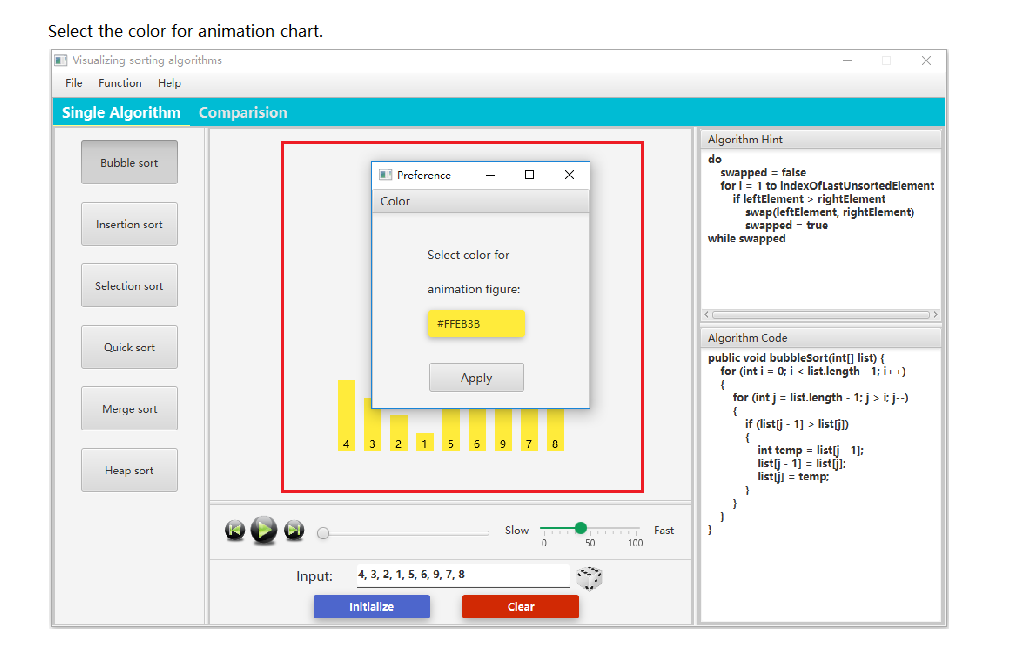
\includegraphics[width=1\textwidth]{user_menu/15.png}
\label{user_menu15}
\end{figure}

\begin{figure}[htbp]
\centering
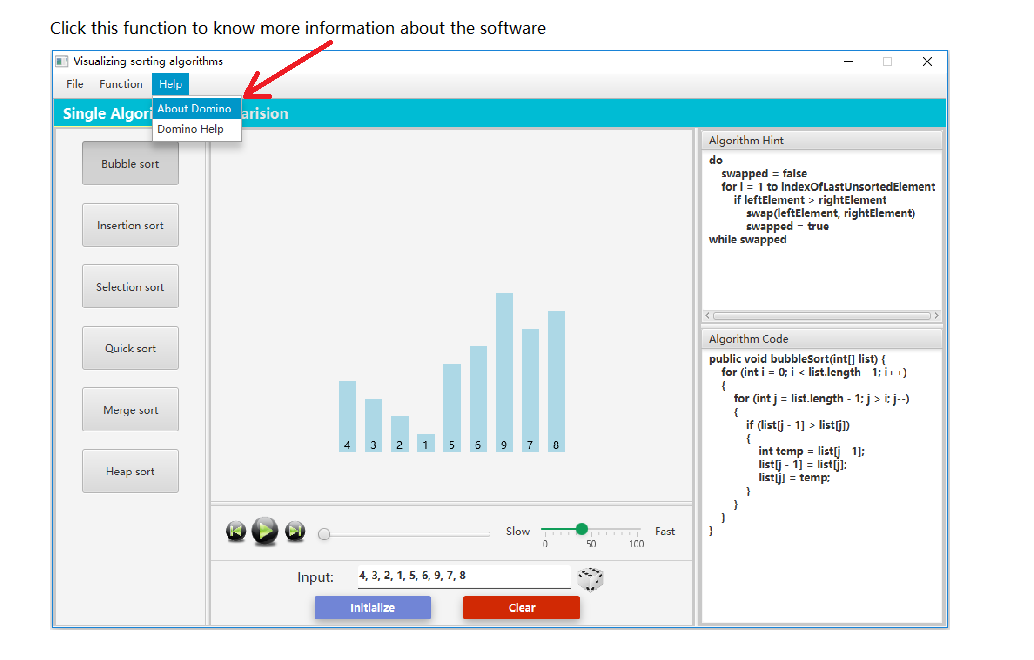
\includegraphics[width=1\textwidth]{user_menu/16.png}
\label{user_menu16}
\end{figure}
\begin{figure}[htbp]
\centering
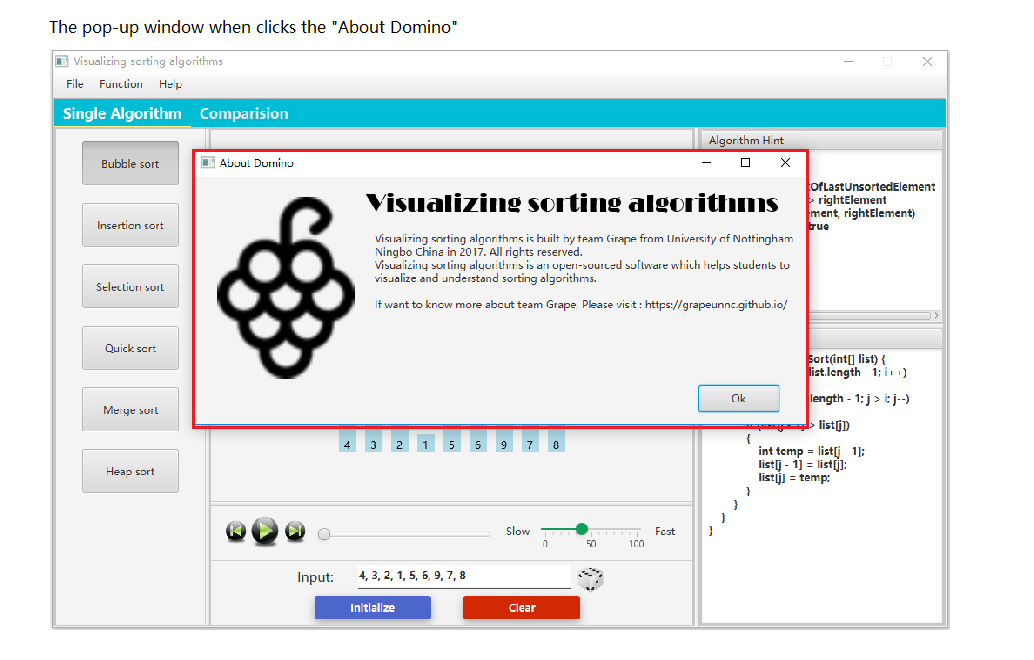
\includegraphics[width=1\textwidth]{user_menu/17.png}
\label{user_menu17}
\end{figure}


\subsection{User Interface Design Update}

\begin{figure}[htbp]
\centering
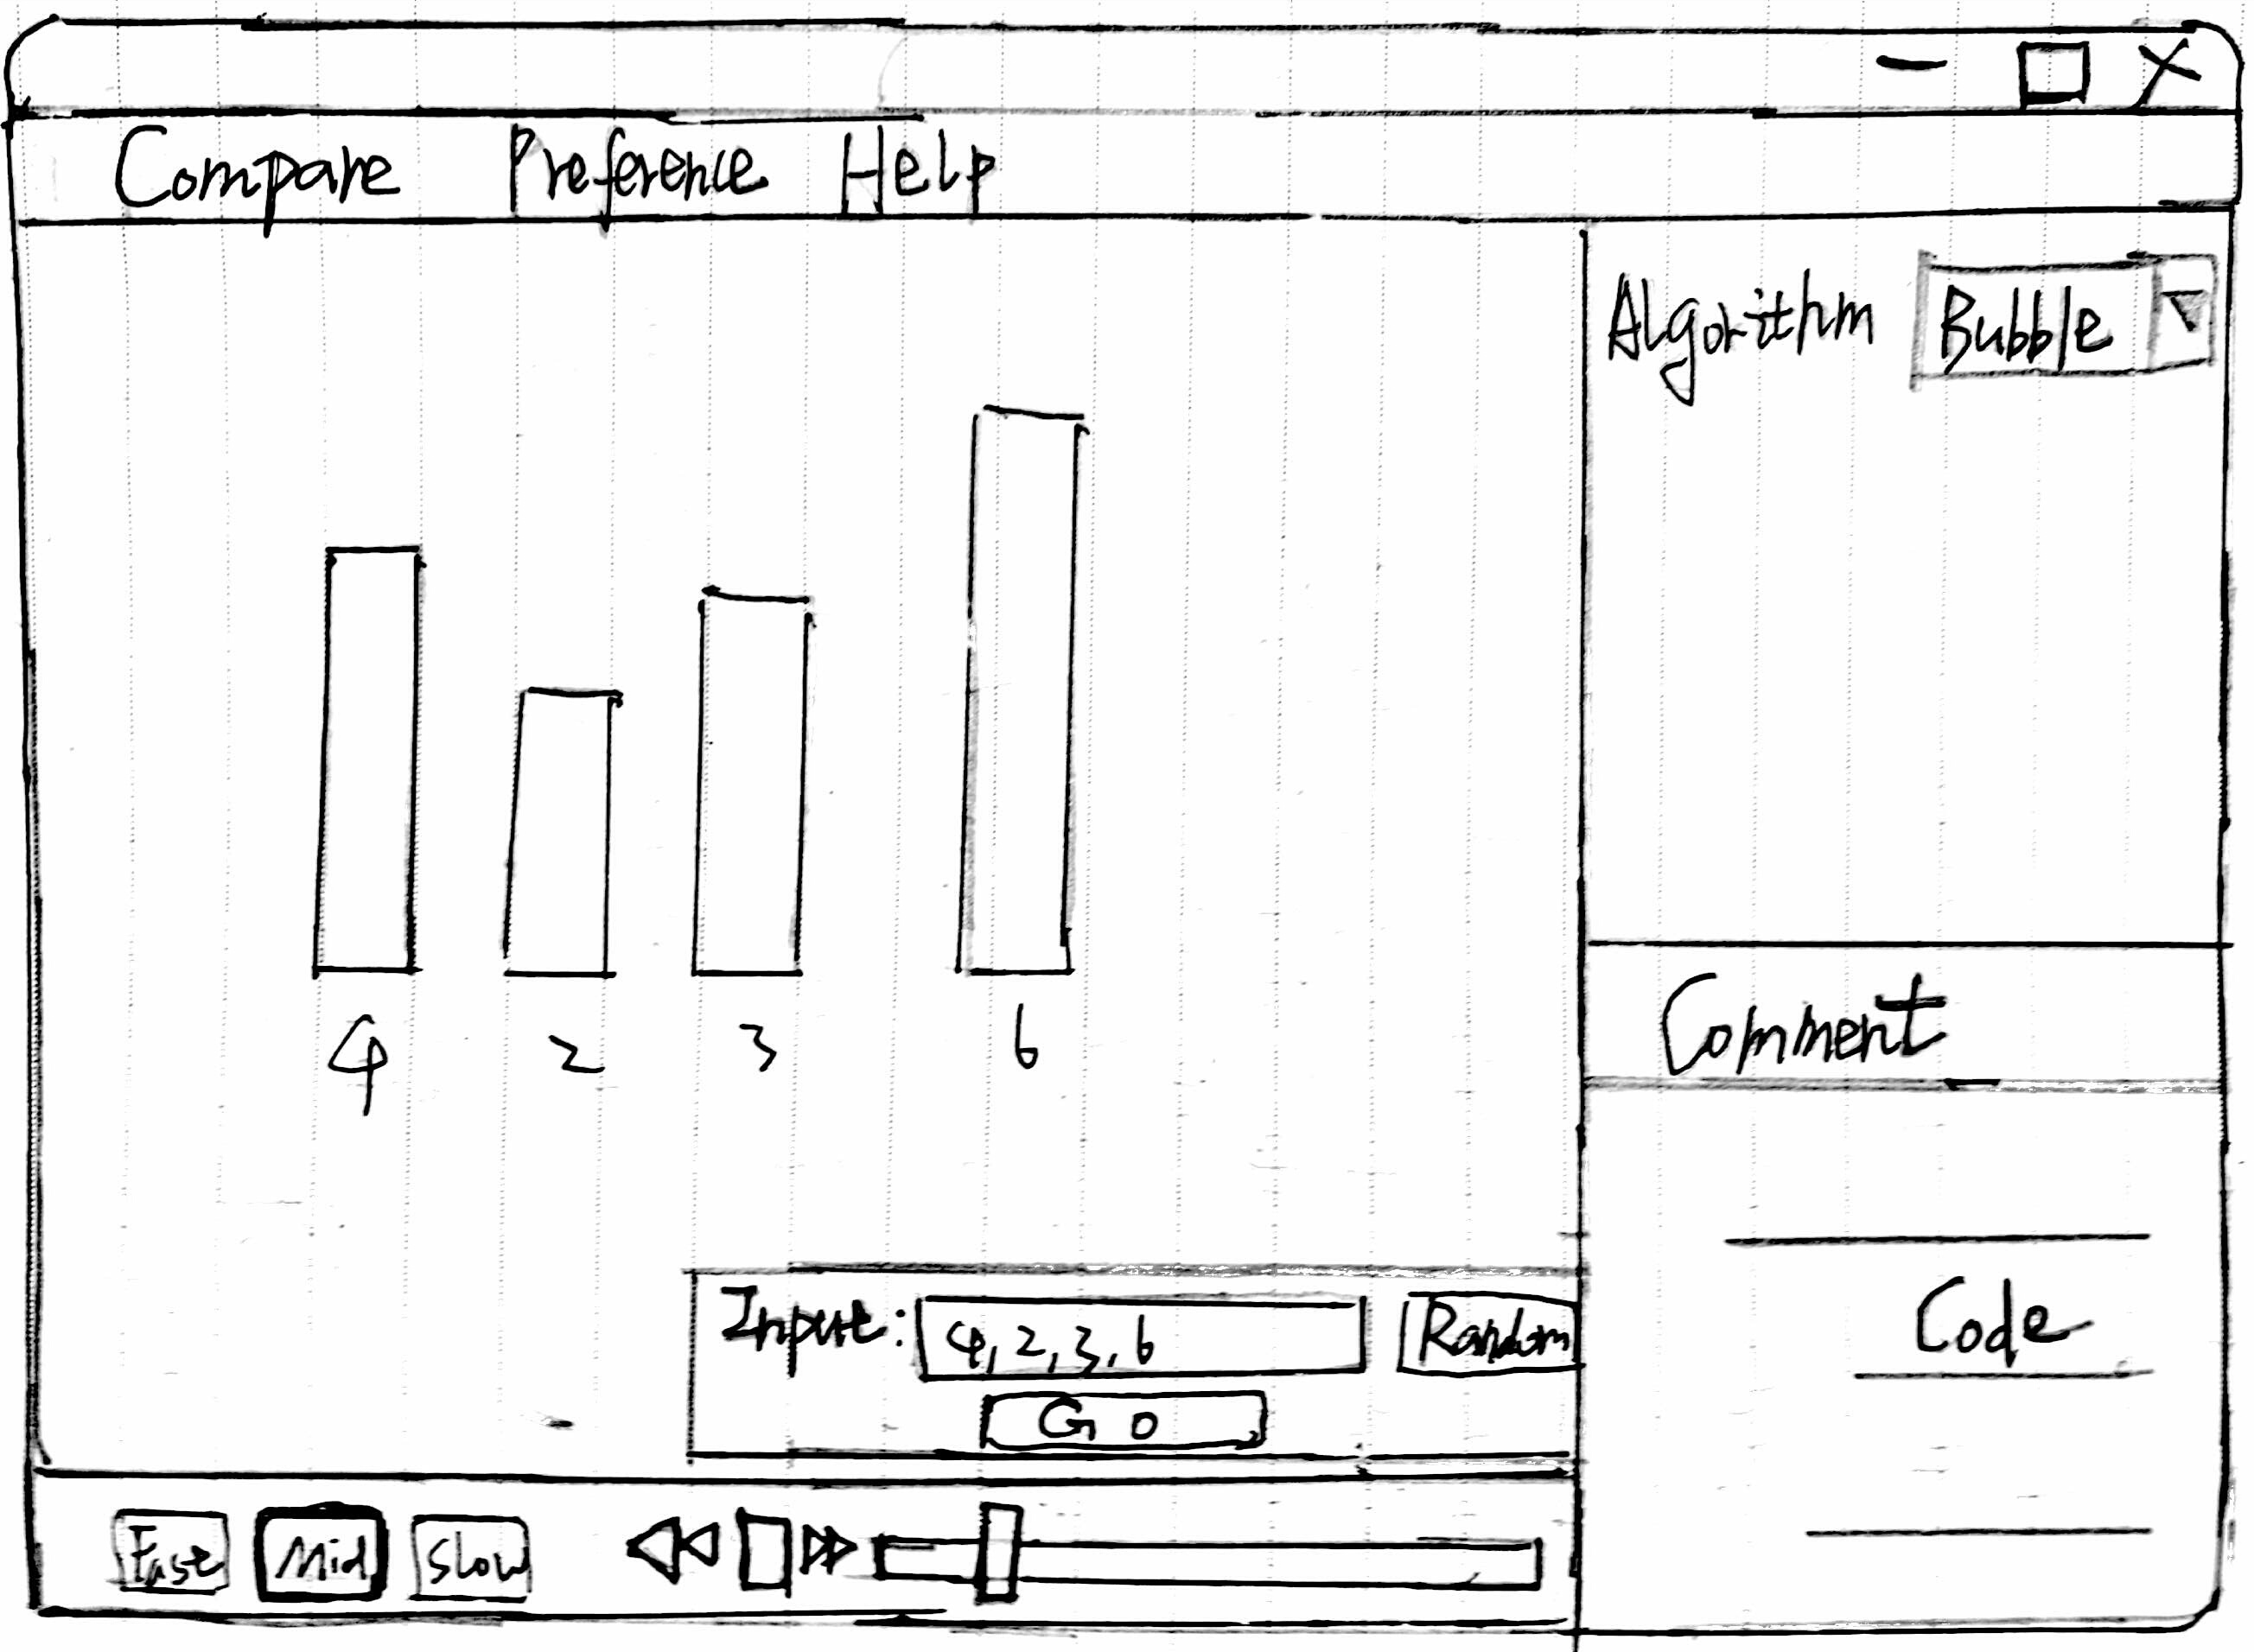
\includegraphics[width=.6\textwidth,height=.4\textwidth]{low-fidelity_prototype.jpg}
\caption{Initial UI Design Scratch}
\label{ui-design}
\end{figure}

\begin{figure}[htbp]
\centering
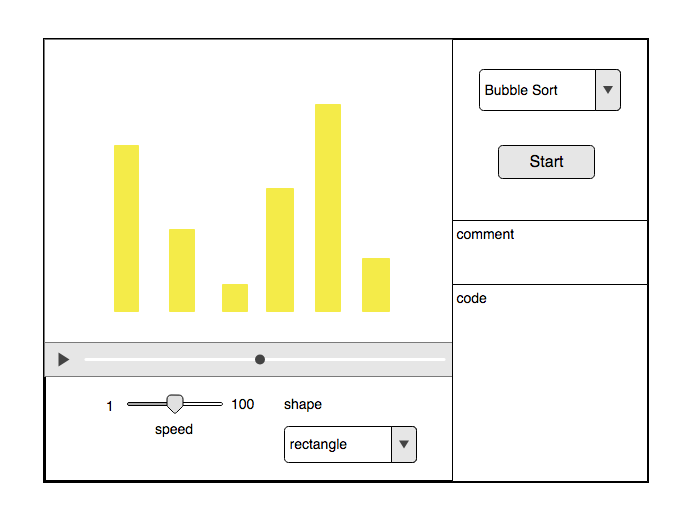
\includegraphics[width=.6\textwidth,height=.4\textwidth]{initialdesign.png}
\caption{Initial UI Design}
\label{initial-design}
\end{figure}

Figure \ref{ui-design} is the initial user interface design. We draw it on the basis of initial requirements. It is simple and crude, but shows the basic idea of the software.

\begin{figure}[htbp]
\centering
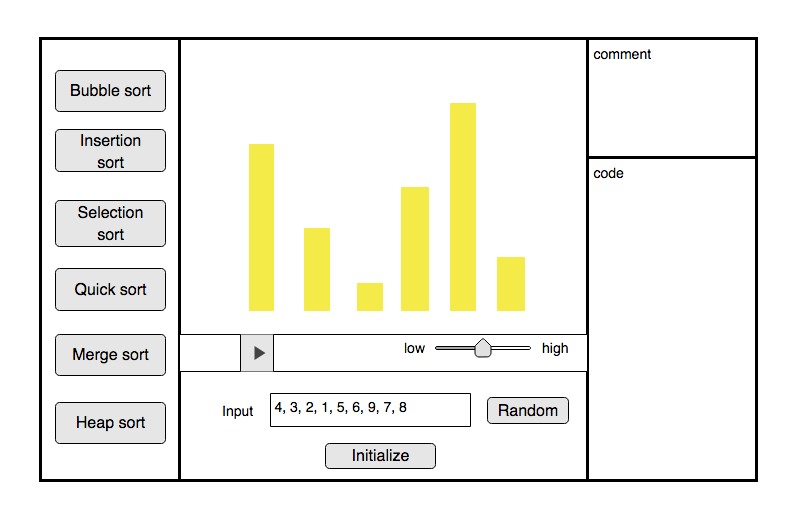
\includegraphics[width=.6\textwidth,height=.4\textwidth]{updateddesign.png}
\caption{updated UI Design}
\label{updated-design}
\end{figure}


\cleardoublepage
% ------------------------------------------------------------------------------
% Bibliography
% ------------------------------------------------------------------------------
\bibliographystyle{unsrtnat}
\bibliography{FinalReport_Grape}

% ------------------------------------------------------------------------------
% End document
% ------------------------------------------------------------------------------
\end{document}
